\chapter[Order and Disorder in Procrystalline Lattices]{Order and Disorder in \\ Procrystalline Lattices} 

\begin{chapterabstract}
Recent work has introduced the term ``procrystalline'' to define systems which lack translational symmetry but have an underlying high symmetry lattice, owing to a difference between the coordination numbers of the molecular units and natural coordination of the underlying lattice.
These materials are expected to exhibit structural properties between crystalline and amorphous phases.
The network properties of a range of these procrystals are investigated, encompassing a range of coordination environments.
Configurations are generated using a zero\--temperature \mc{} method, whilst simpler lattices are also considered analytically.
Procrystals are shown to be rare examples of systems with violate \lm{}'s law, whilst also displaying assortativities different to those calculated for amorphous materials.
Procrystalline lattices are therefore shown to have fundamentally different behaviour to traditional disordered and crystalline systems, indicative of the partial ordering of the underlying lattices.
\end{chapterabstract}

\section{The Procrystalline State}

Investigations into inorganic network\--forming materials have led to the introduction of the term ``procrystalline'' to refer to systems in which molecular building blocks lie on a regular array of lattice points, but directional interactions lead to overall correlated disorder \cite{Overy2016}.
As an introductory example, consider the procrystal in figure \ref{fig:prointroa}.
In this configuration the nodes form a square net, but each lattice site is occupied by a ``T'' shaped unit.
If the ends of these units are mutually attractive, they will orient to maximise favourable interactions.
The consequence of this is to introduce disorder into the ring structure.
This can be detected in the dual network, as in figure \ref{fig:prointrob}, which in this case can be viewed as a defective square net.
More strikingly, a system of percolating rings once again emerges, highlighted in figure \ref{fig:prointroc}, in analogue with networks from previous chapters. 

\begin{figure}[bt]
     \centering
     
     \begin{subfigure}[b]{0.3\textwidth}
         \centering
         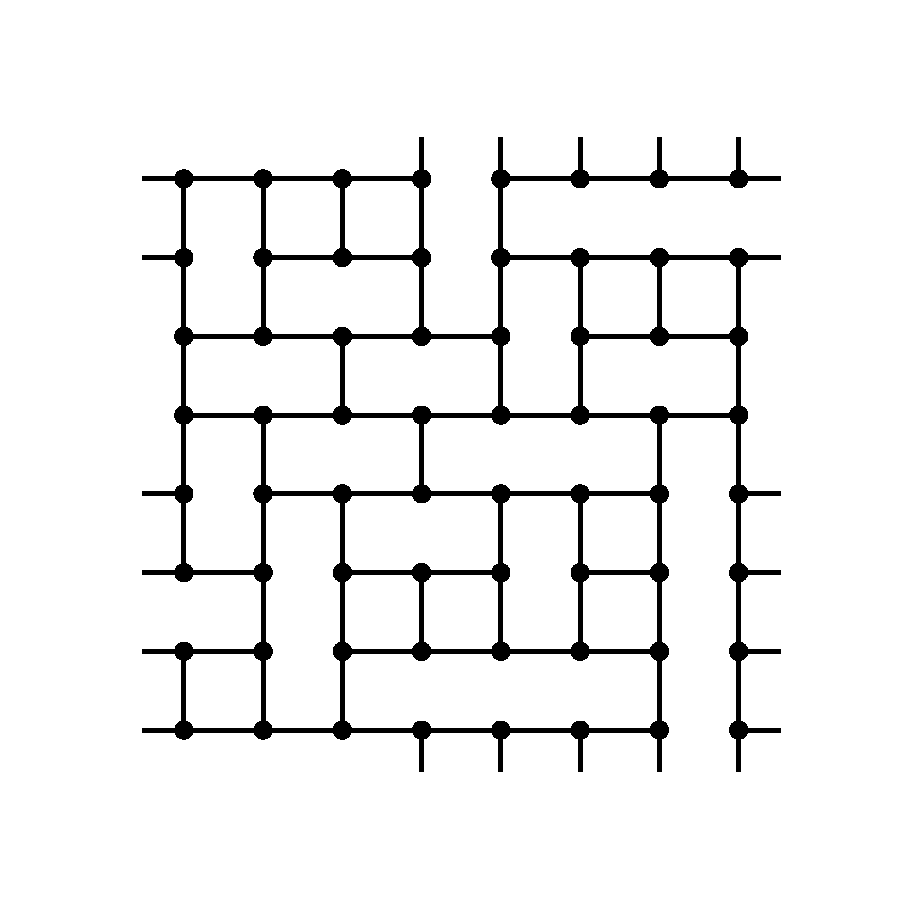
\includegraphics[width=\textwidth]{./figures/procrystals/pro_intro3.pdf}
         \caption{Procrystalline lattice}
         \label{fig:prointroa}
     \end{subfigure}
     \hfill
      \begin{subfigure}[b]{0.3\textwidth}
         \centering
         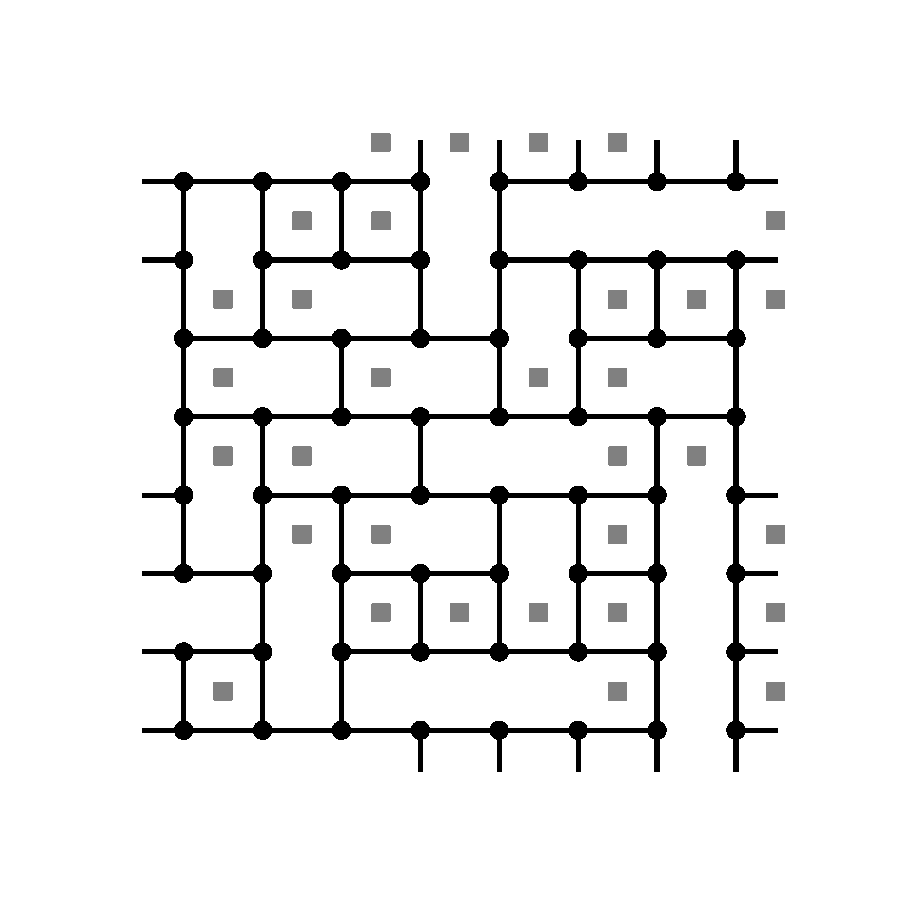
\includegraphics[width=\textwidth]{./figures/procrystals/pro_intro1.pdf}
         \caption{Overlay with dual}
         \label{fig:prointrob}
     \end{subfigure}
     \hfill
     \begin{subfigure}[b]{0.3\textwidth}
         \centering
         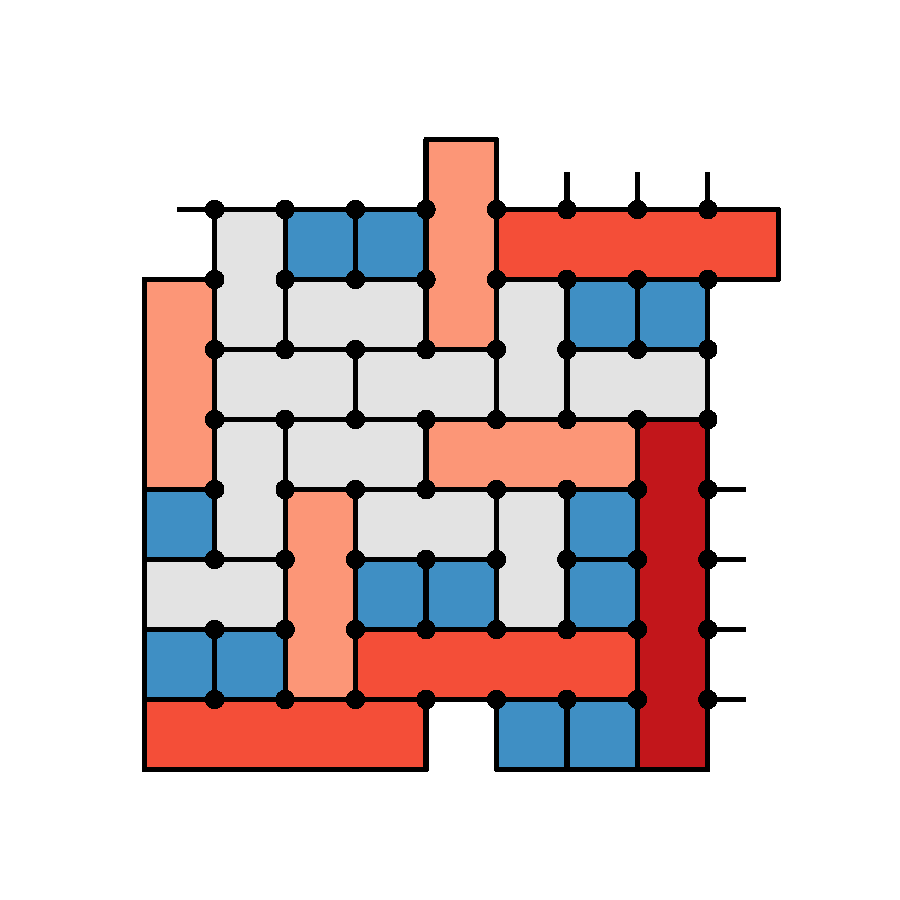
\includegraphics[width=\textwidth]{./figures/procrystals/pro_intro2.pdf}
         \caption{Ring structure}
         \label{fig:prointroc}
     \end{subfigure}
     
     \caption{Example procrystalline lattice based on the square net. Panel (a) shows the lattice with each node representing a 3\--coordinate molecular unit. Panel (b) adds the nodes of the dual network, which form a defective square lattice. Panel (c) highlights the corresponding ring structure, coloured by ring size.}
     \label{fig:nprointro}
\end{figure}

The local environment around each node in a procrystal is therefore identical, leading them to appear crystalline in their atomic RDFs and structure factors. 
However, considering the network in its entirety with both nodes and links, it is clear an infinite procrystalline lattice has no unit cell.
As such procrystals can be considered to sit somewhere in between traditional crystals and the amorphous materials discussed in previous chapters.
This ``partial disordering'' is expected to be reflected in their structural and electronic properties.

Experimentally there are several systems which can be thought of as realisations of procrystals. 
These include self-assembled molecular monolayers, classical bond valence solids, mixed-anion perovskites, and order/disorder ferroelectrics \cite{Blunt2008,Anderson1973,Camp2012,Comes1968}.
Whilst this list is not extremely extensive (particularly for \td{} examples), it demonstrates the diversity in the range of potential structures that can form procrystals.
Again although the future focus of the field may be lie more in three\--dimensional structures, the constraints and simplifications that arise from reduced dimensionality make \td{} structures the natural starting place for investigations into the properties of these procrystalline materials.

\section{Two\--Dimensional Procrystalline Lattices}

In this chapter a range of \td{} procrystalline systems will be investigated based on a selection of underlying high symmetry lattices and node coordination numbers.
Figure \ref{fig:symlat} details the high symmetry lattices that form the basis of these procrystals.
These regular and semi\--regular tilings have been chosen to provide a series of underlying coordination numbers in the range $4\rightarrow6$, whilst also occurring across various theoretical and experimental studies on \td{} materials.
The $4$\--coordinate tilings considered are the square \cite{Algara-Siller2015,Zhu2017,Hibble2011} and trihexagonal (also known as kagome) \cite{Zheng2014,Postulka2016,Chen2011} nets,
the $5$\--coordinate tilings are the elongated\--triangular \cite{Griffith2018} and snub\--square \cite{Urgel2014,Kryuchkov2018,Song2015,Pineros2016} nets, and the $6$\--coordinate tiling is the triangular net. 

\begin{figure}[bt]
     \centering
     
     \begin{subfigure}[b]{0.3\textwidth}
         \centering
         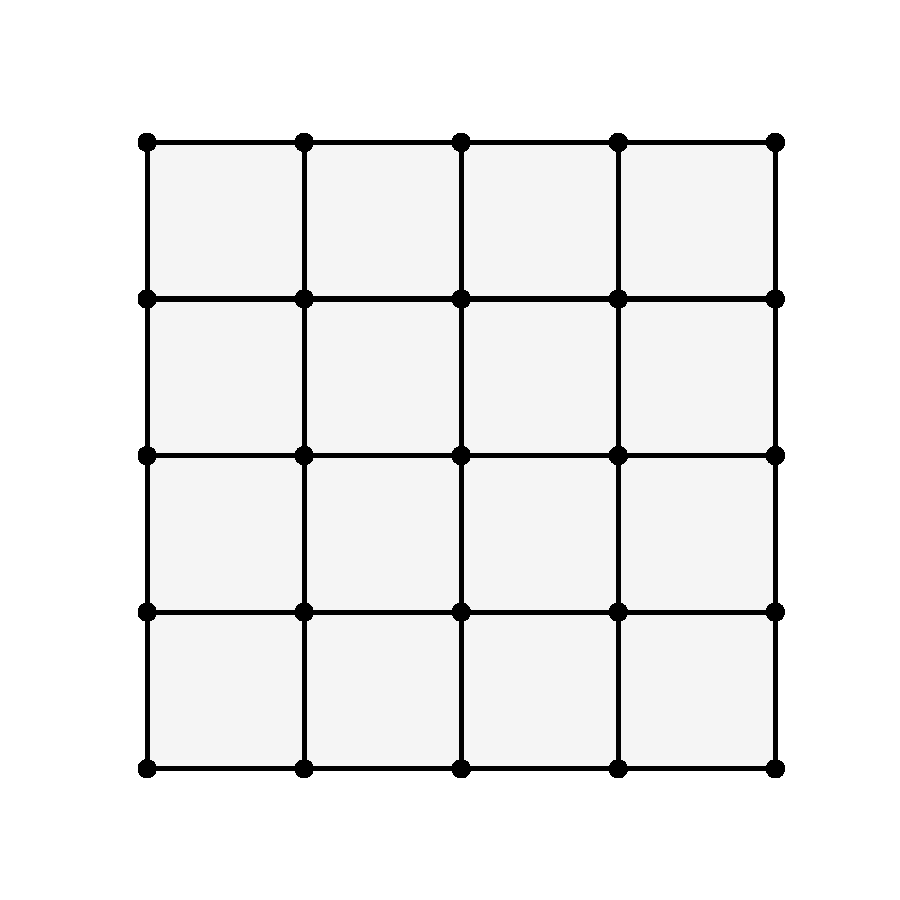
\includegraphics[height=2.5cm]{./figures/procrystals/sq.pdf}
         \caption{Square}
         \label{fig:symlatsq}
     \end{subfigure}
     \begin{subfigure}[b]{0.3\textwidth}
         \centering
         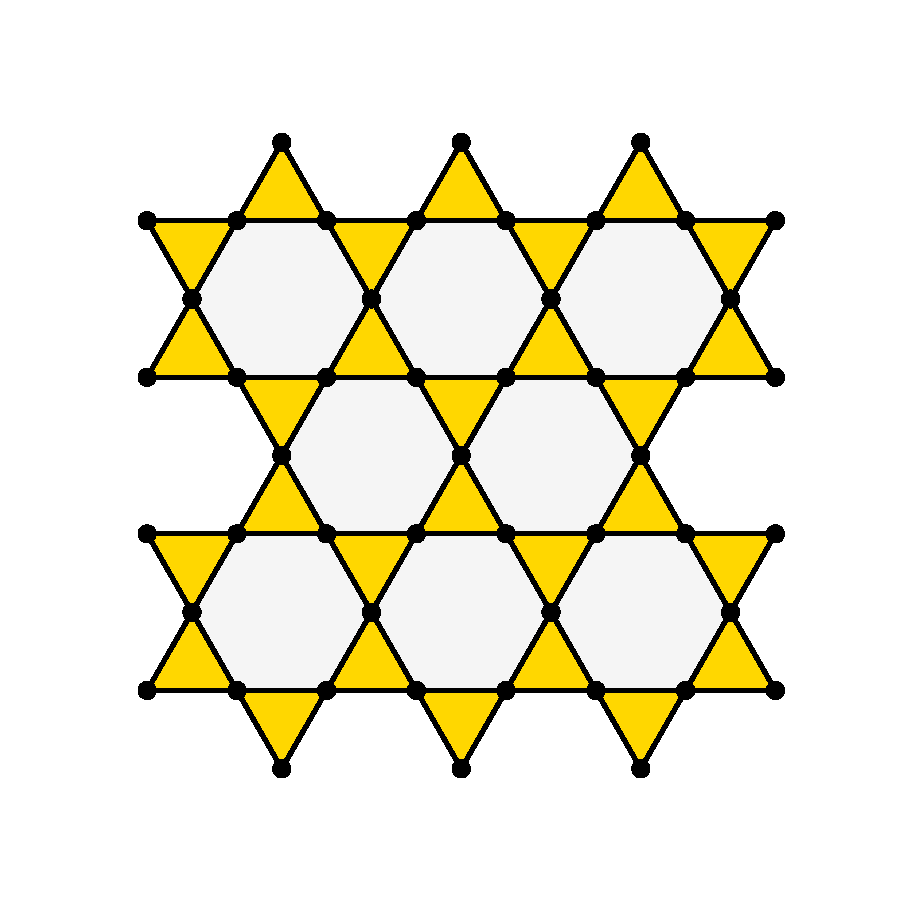
\includegraphics[height=2.5cm]{./figures/procrystals/trihex.pdf}
         \caption{Trihexagonal (kagome)}
         \label{fig:symlattrihex}
     \end{subfigure}
     \hfill
     
     \vspace{0.5cm}
     
     \begin{subfigure}[b]{0.3\textwidth}
         \centering
         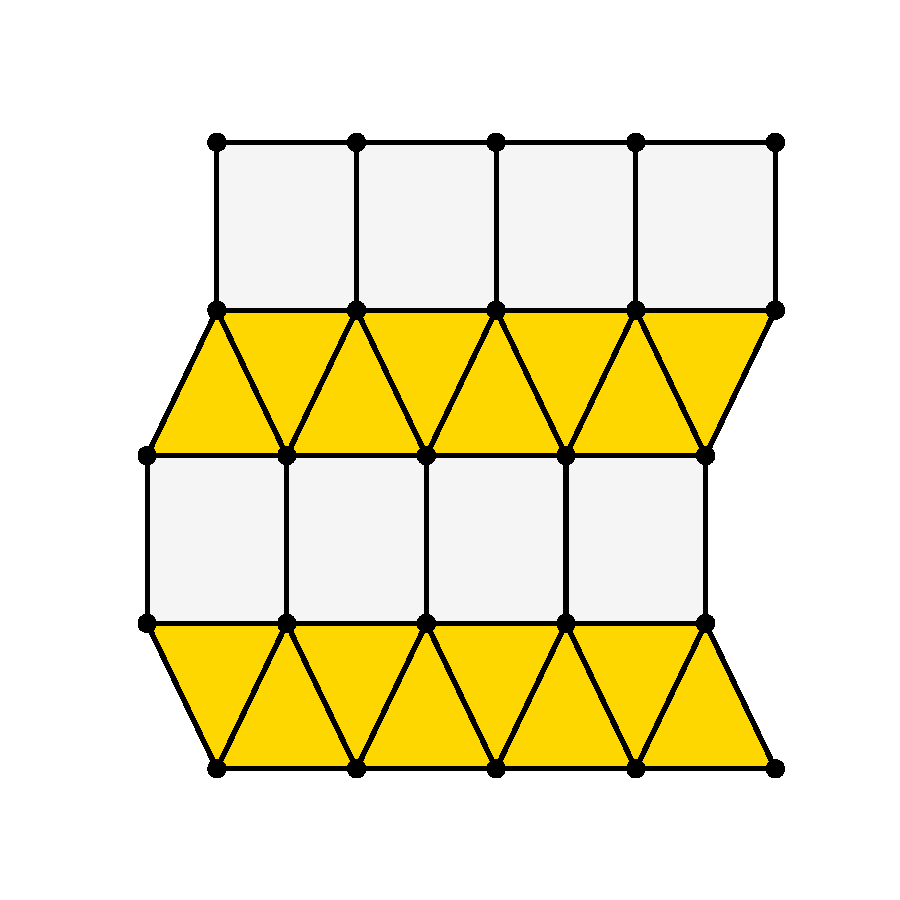
\includegraphics[height=2.5cm]{./figures/procrystals/elongtri.pdf}
         \caption{Elongated\--triangular}
         \label{fig:symlatelong}
     \end{subfigure}
     \begin{subfigure}[b]{0.3\textwidth}
         \centering
         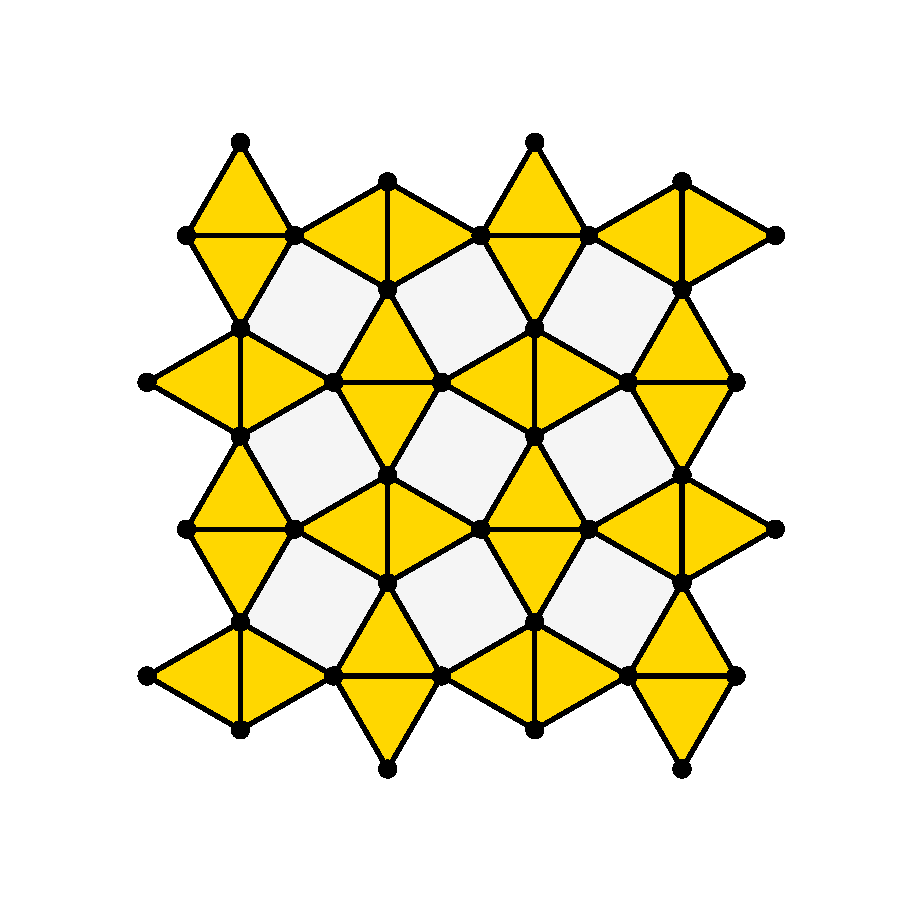
\includegraphics[height=2.5cm]{./figures/procrystals/snub.pdf}
         \caption{Snub\--square}
         \label{fig:symlatsnub}
     \end{subfigure}
     \hfill
     
     \begin{subfigure}[b]{0.3\textwidth}
         \centering
         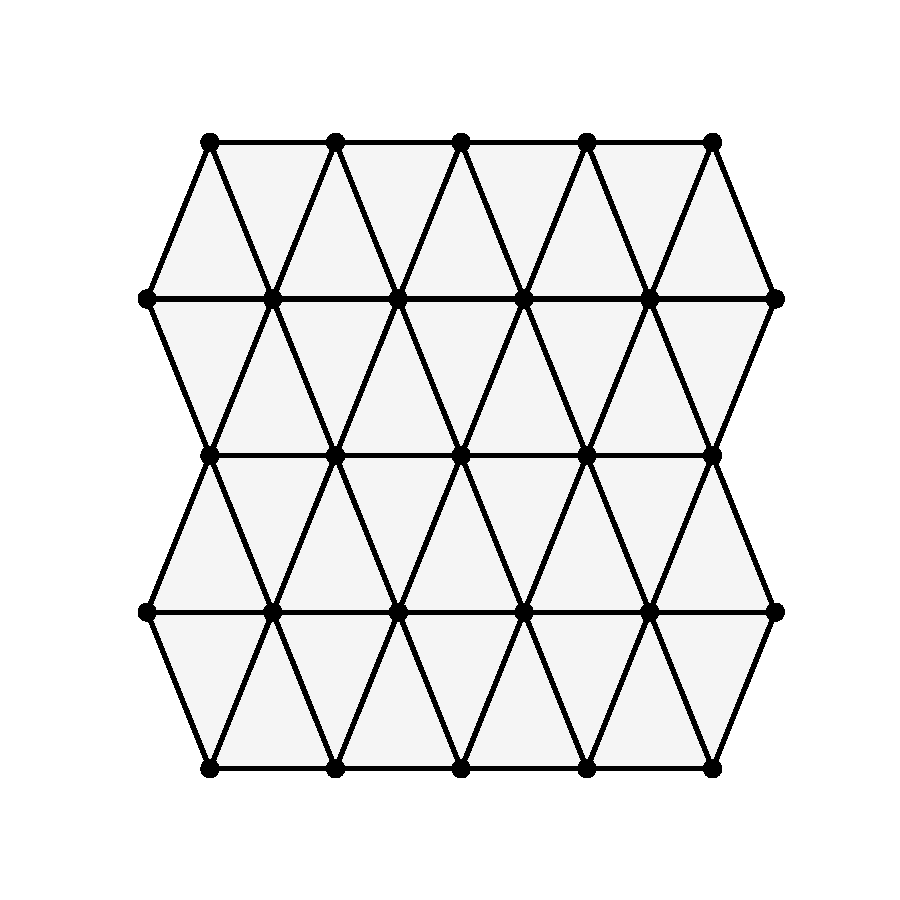
\includegraphics[height=2.5cm]{./figures/procrystals/tri.pdf}
         \caption{Triangular}
         \label{fig:symlattri}
     \end{subfigure}
     \hfill

     \caption{High symmetry lattices that form the basis of \td{} procrystalline lattices in this work. The square and trihexagonal lattices (panels (a), (b)) have a natural coordination number of 4; the elongated triangular and snub square lattices (panels (c), (d))  of 5 and the triangular lattice (panel (e)) of 6.}
     \label{fig:symlat}
\end{figure}

The disorder in procrystals arises from the discrepancy between the natural coordination numbers of the regular lattice and the actual coordination of the nodes which occupy them.
If the coordination of these high symmetry ``parent'' lattices is denoted $c^\prime$, it follows that each is is able to generate procrystalline lattices with node coordinations, $c$, in the range $c=3\rightarrow \left(c^\prime-1\right)$ (strictly 2\--coordinate procrystals are also obtainable, but these form ``spaghetti'' like structures with ill defined ring structure \cite{Baise2018}).
In this thesis, for simplicity these procrystals will be referred to with the notation \pro{c^\prime}{c}lattices.
In addition, whilst for \pro{c^\prime}{\left(c^\prime-1\right)}lattices there is only one possible way of arranging the $c^\prime-1$ links around each node, for the other lattices this is not the case.
As a simplification it will be assumed that all arrangements are possible and equally likely.

\subsection{Network Measures}

Procrystals can be considered as additional examples of the tessellating ring structures seen in previous chapters, the difference being that the ring geometries are constrained by the underlying lattice. 
As such the network measures discussed previously are also applicable to procrystalline lattices.  
For instance, procrystals are subject to Euler's formula such that the mean ring size is constrained by equation \eqref{eq:avdegree}.

When discussing the maximum entropy ring size distributions, a similar approach can be taken as for \lm's law (see section \ref{s:lemaitre}), save constraint \eqref{con:lm3} no longer applies.
To get the expected maximum entropy ring statistics, $\pme_k$, one can remove this constraint to give a simple modification of equation \eqref{eq:mepk}:
\begin{equation}
	\label{eq:prome}
    \pme_k = \frac{e^{-\lambda k}}{\sumk e^{-\lambda k}}\,.
\end{equation}
As with \lm's law, an important additional constraint arises implicitly through the $k$\--range in the summation.
Owing to the fact that there are many subtly different systems here, these will be further discussed in the relevant sections \davidnote{link}.

Finally, the assortativity will again be used to measure ring\--ring correlations. \davidnote{ref}

\section{Computational Generation of Procrystals}

Although experimental procrystalline lattices are aperiodic with no unit cell, computational studies are naturally restricted in scope and an effective way of generating lattices with fully satisfied valence is to reintroduce periodicity. 
%In addition, configurations which are divided in two \ie{} have two disconnected components are neglected
There are then two possible ways to proceed in order to map the configurational space of procrystals.
Firstly, one can attempt to find all possible arrangements for a lattice of given size, which here is termed \textit{exact tiling}.
Whilst exact tiling gives a complete view of the procrystalline landscape, it will be seen that even with optimisations it quickly becomes computationally intractable.

The second approach is to sample configurations using a stochastic method such as \mc{} sampling.
This allows procrystalline configurations to be generated which are representative of the wider landscape for far larger lattice dimensions.
This has the advantage of mitigating any effects of enforcing periodicity, and will be the primary method used to generate procrystals in this work.

\subsection{Exact Tiling Algorithm}

The exact tiling algorithm finds all procrystalline lattices for a given lattice dimension using a divide\--and\--conquer approach.
It has been used here to investigate the \pro{4}{3}square lattice.
The method starts from the observation that there are seven possibilities for each square in the procrystalline lattice (some of which are symmetry related) forming the $1\times 1$ tiles in figures \ref{fig:et1x1_0}\--\ref{fig:et1x1_6} (these are colour coded by a central circle).
These $1\times 1$ tiles can be stacked to produce $1\times 2$ tiles, of which there are 22 possibilities that satisfy internal coordination requirements (but are not necessarily periodic), the first 5 of which are given in figures \ref{fig:et2x1_0}\--\ref{fig:et2x1_4}.
Again these can in turn be stacked to yield 84 $2\times 2$ building blocks, a selection of which are given in figures \ref{fig:et2x2_0}\--\ref{fig:et2x2p_3}.

\begin{figure}[bt]
     \centering
     
     \begin{subfigure}[b]{0.1\textwidth}
         \centering
         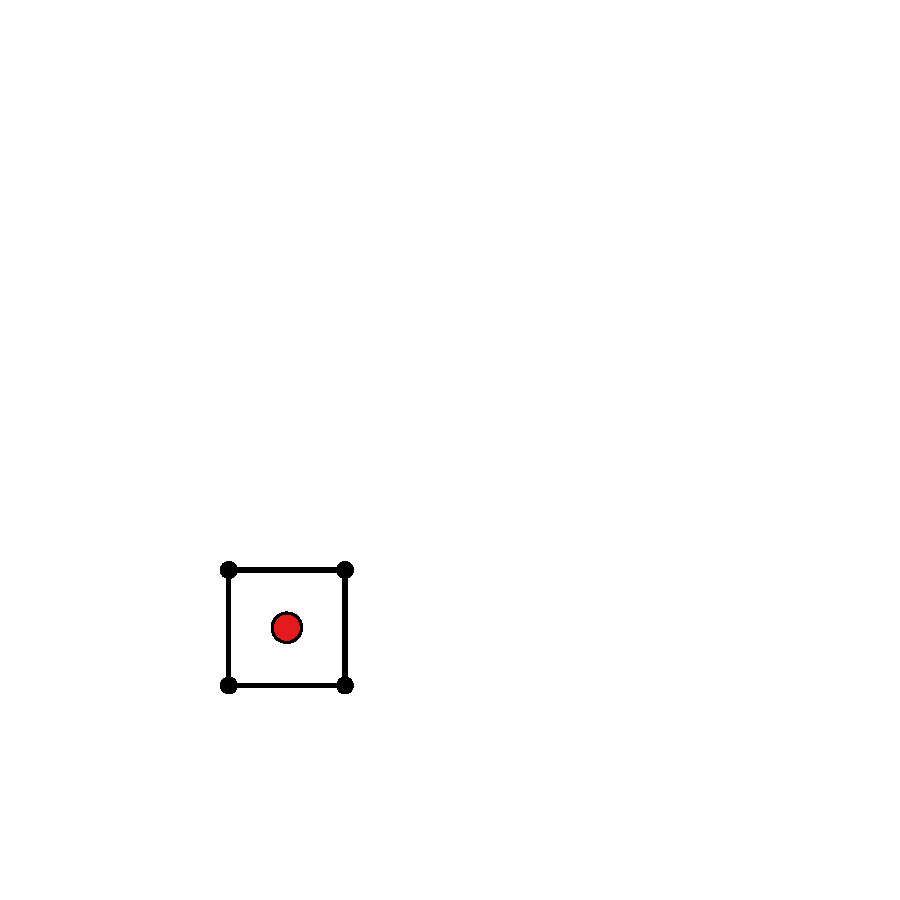
\includegraphics[height=1.2cm]{./figures/procrystals/1x1_0.pdf}
         \caption{}
         \label{fig:et1x1_0}
     \end{subfigure}
     \hfill
     \begin{subfigure}[b]{0.1\textwidth}
         \centering
         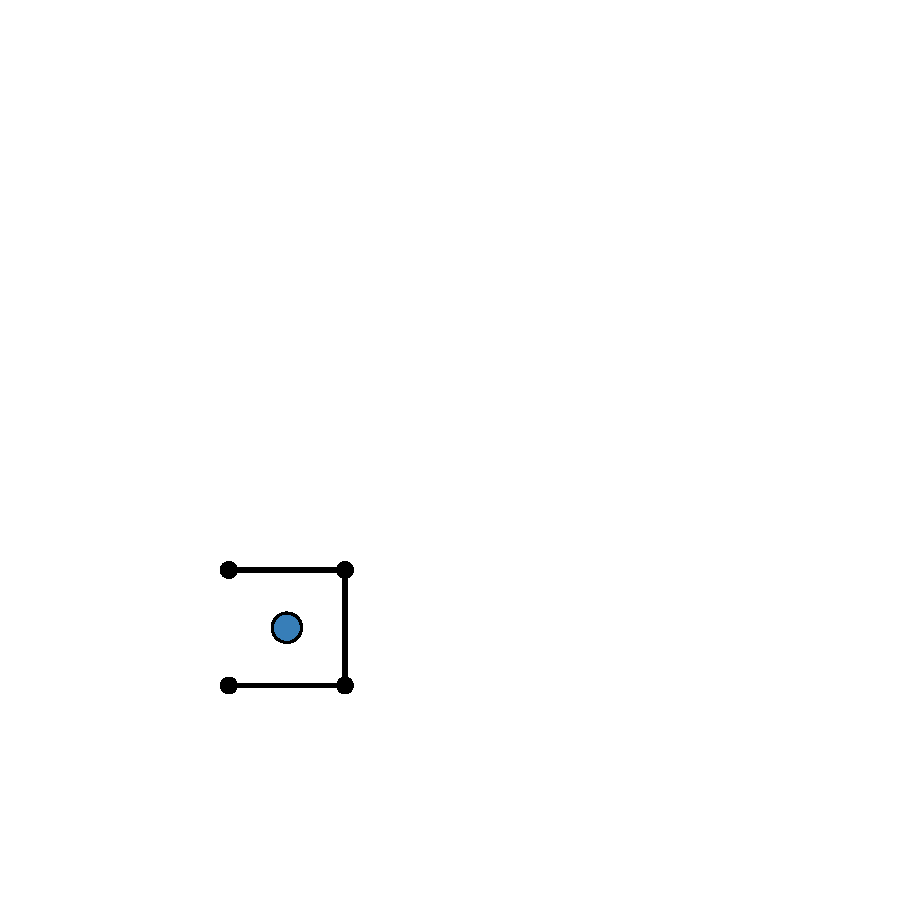
\includegraphics[height=1.2cm]{./figures/procrystals/1x1_1.pdf}
         \caption{}
         \label{fig:et1x1_1}
     \end{subfigure}
     \hfill
     \begin{subfigure}[b]{0.1\textwidth}
         \centering
         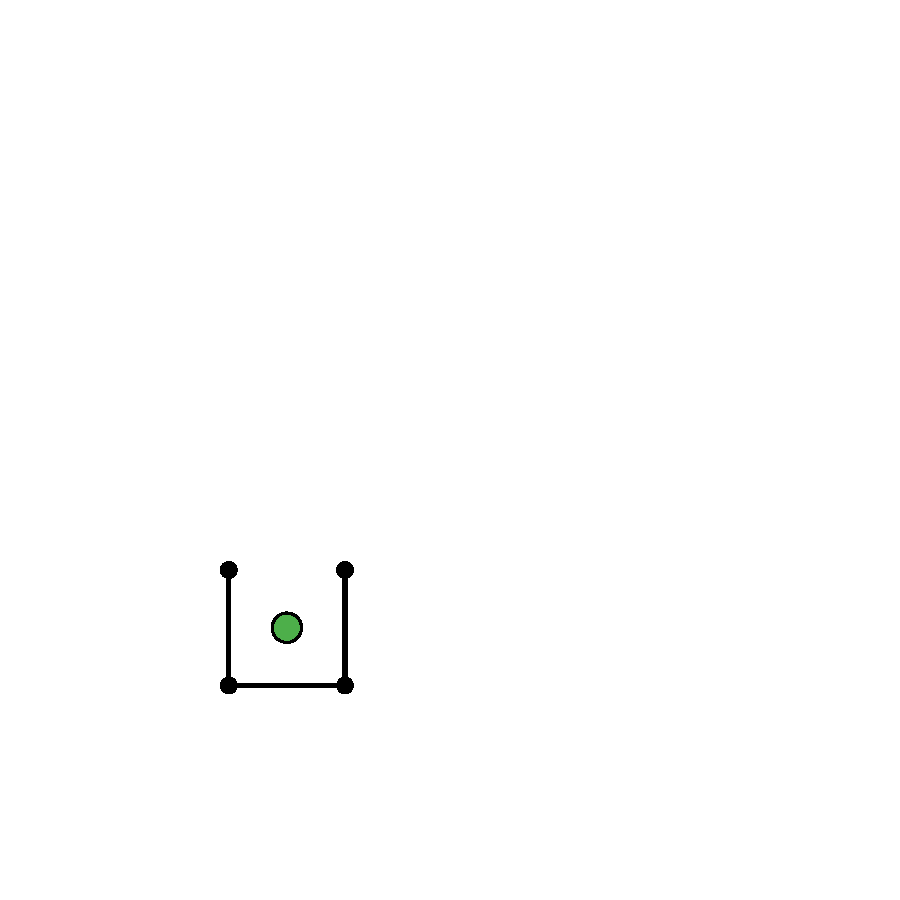
\includegraphics[height=1.2cm]{./figures/procrystals/1x1_2.pdf}
         \caption{}
         \label{fig:et1x1_2}
     \end{subfigure}
     \hfill
     \begin{subfigure}[b]{0.1\textwidth}
         \centering
         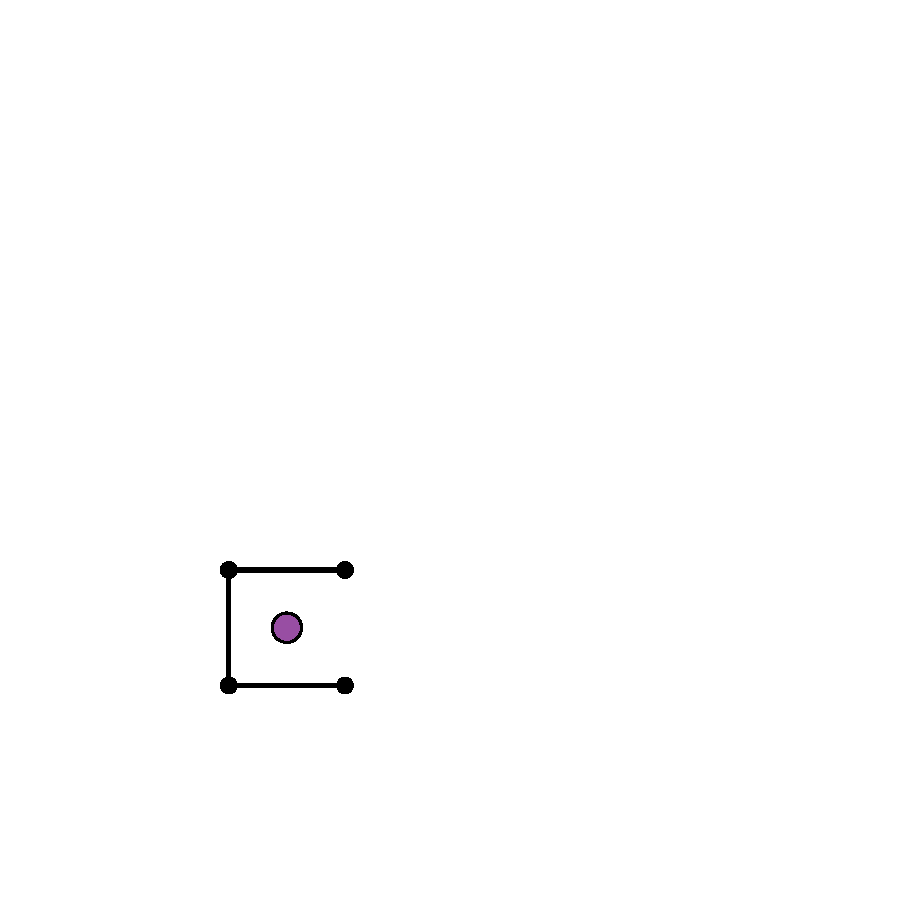
\includegraphics[height=1.2cm]{./figures/procrystals/1x1_3.pdf}
         \caption{}
         \label{fig:et1x1_3}
     \end{subfigure}
     \hfill
     \begin{subfigure}[b]{0.1\textwidth}
         \centering
         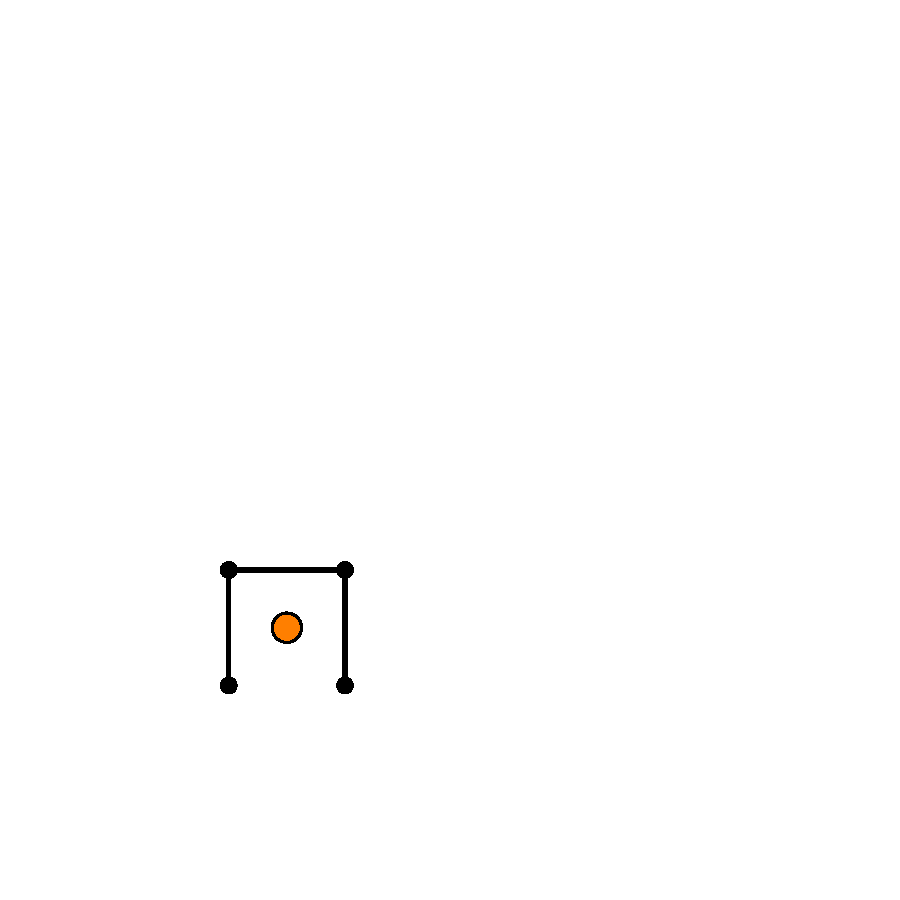
\includegraphics[height=1.2cm]{./figures/procrystals/1x1_4.pdf}
         \caption{}
         \label{fig:et1x1_4}
     \end{subfigure}
     \hfill
     \begin{subfigure}[b]{0.1\textwidth}
         \centering
         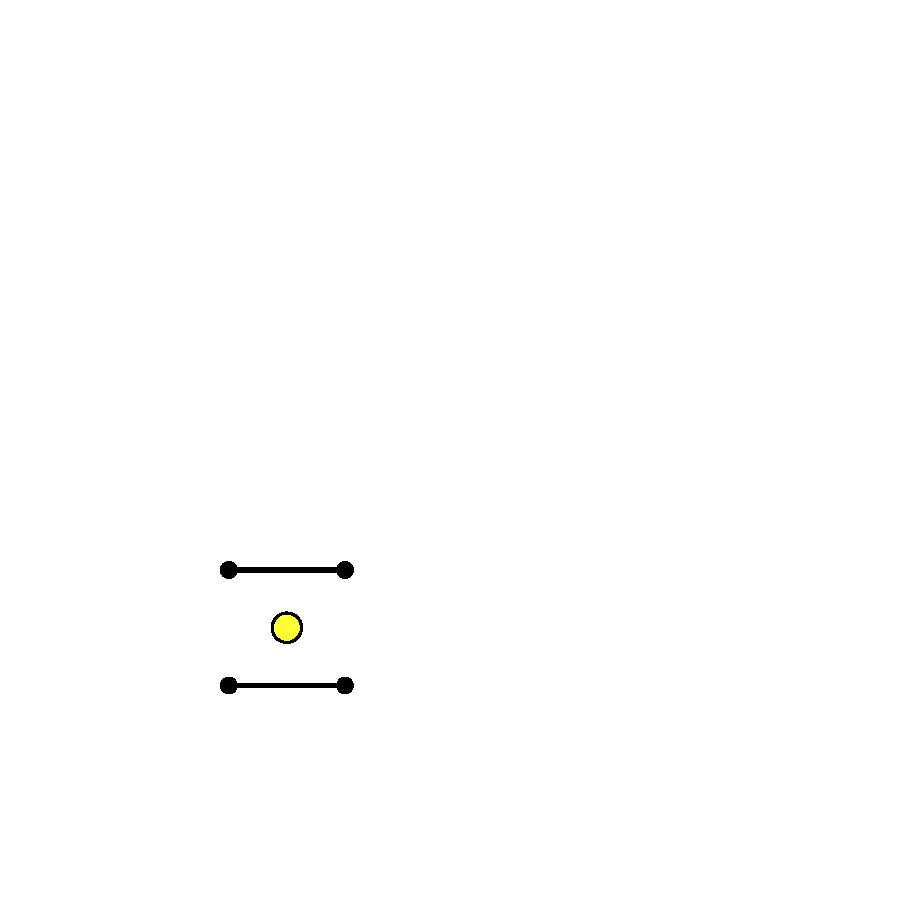
\includegraphics[height=1.2cm]{./figures/procrystals/1x1_5.pdf}
         \caption{}
         \label{fig:et1x1_5}
     \end{subfigure}
     \hfill
     \begin{subfigure}[b]{0.1\textwidth}
         \centering
         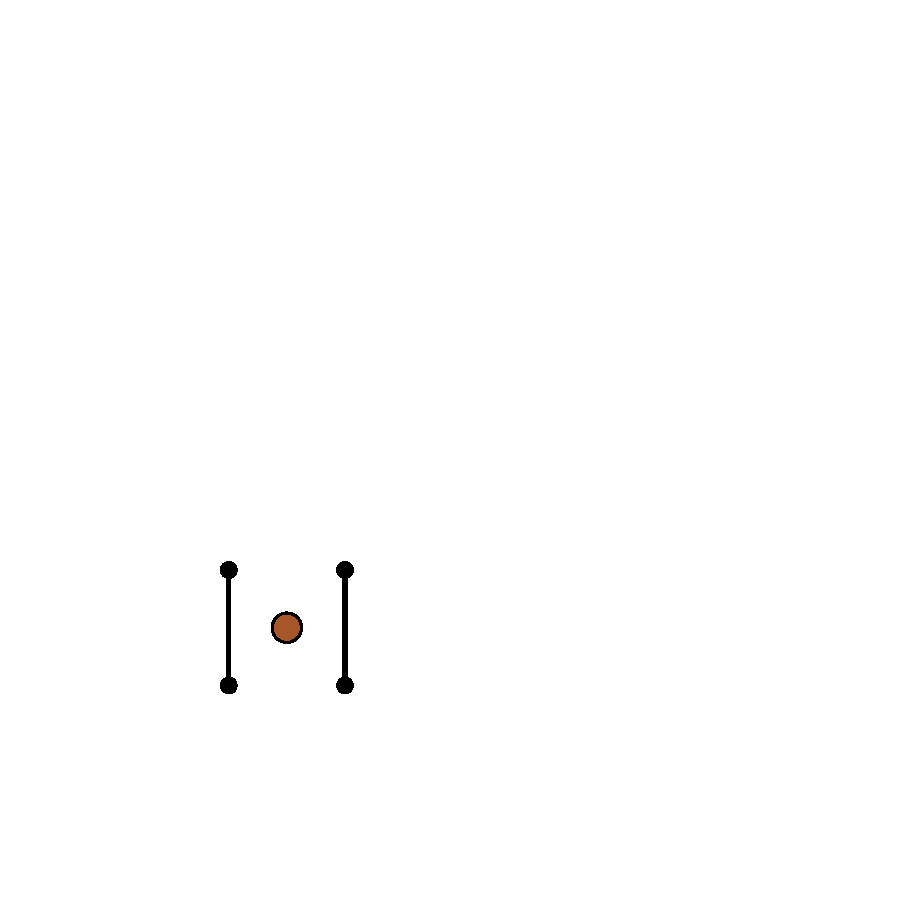
\includegraphics[height=1.2cm]{./figures/procrystals/1x1_6.pdf}
         \caption{}
         \label{fig:et1x1_6}
     \end{subfigure}
     \hfill
     \vspace{0.5cm}
     
     \begin{subfigure}[b]{0.19\textwidth}
         \centering
         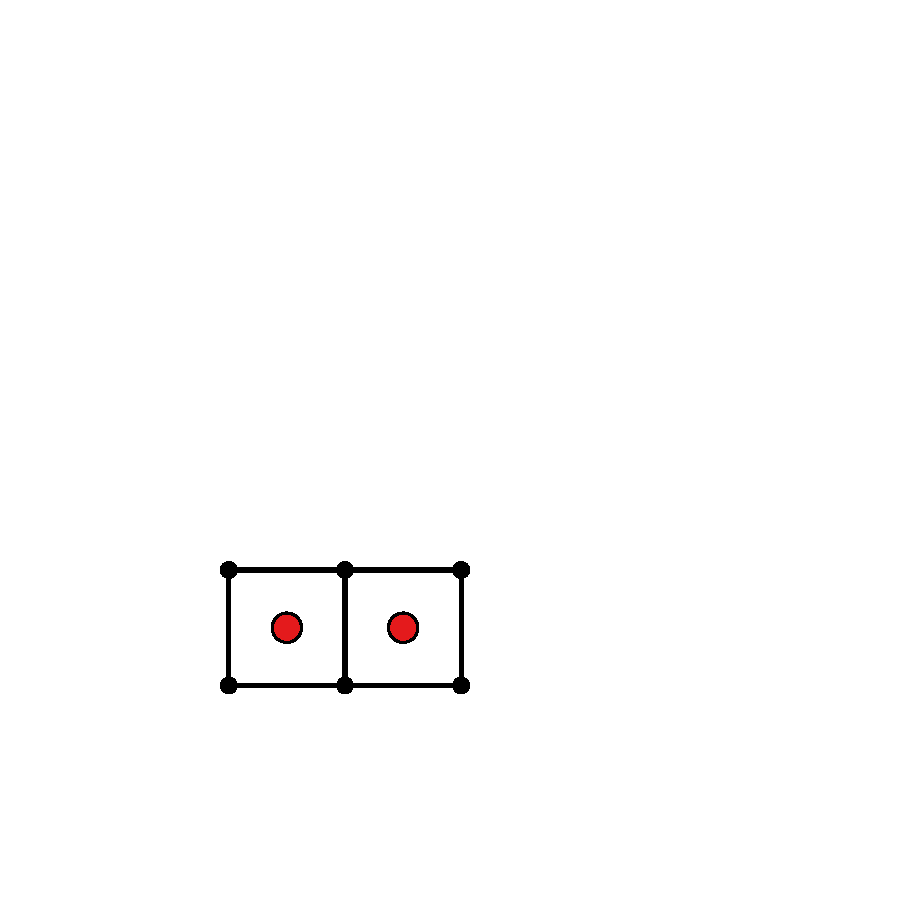
\includegraphics[height=1.2cm]{./figures/procrystals/2x1_0.pdf}
         \caption{}
         \label{fig:et2x1_0}
     \end{subfigure}
     \hfill
     \begin{subfigure}[b]{0.19\textwidth}
         \centering
         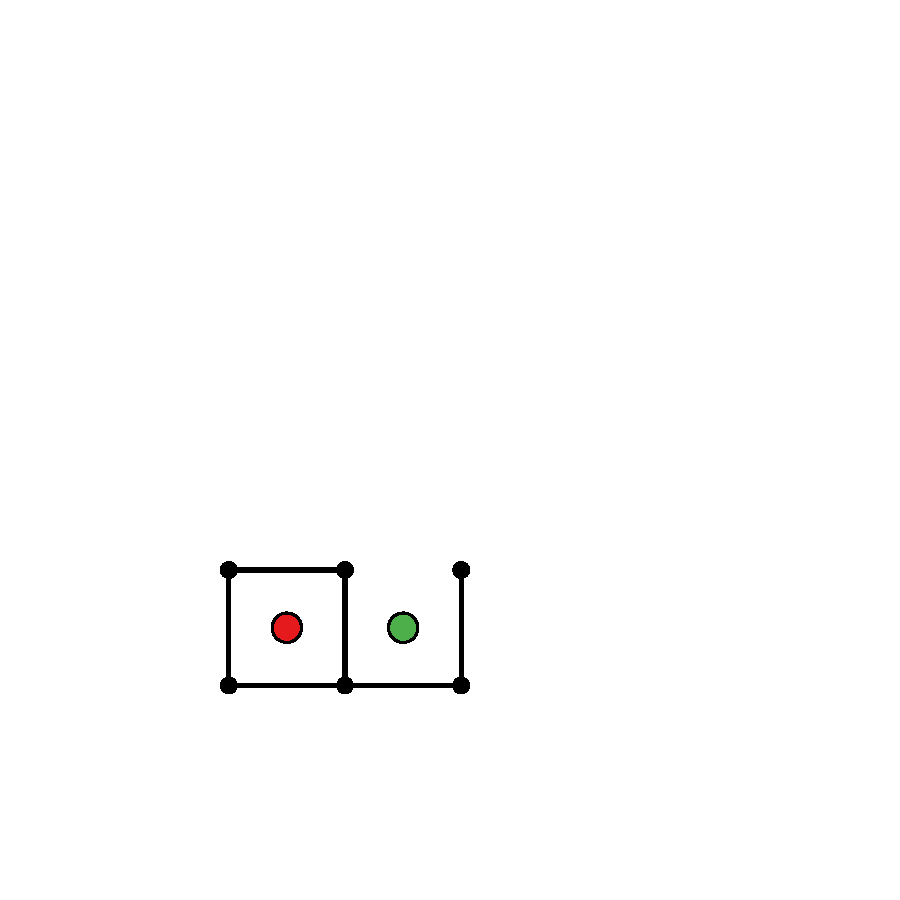
\includegraphics[height=1.2cm]{./figures/procrystals/2x1_1.pdf}
         \caption{}
         \label{fig:et2x1_1}
     \end{subfigure}
     \hfill
     \begin{subfigure}[b]{0.19\textwidth}
         \centering
         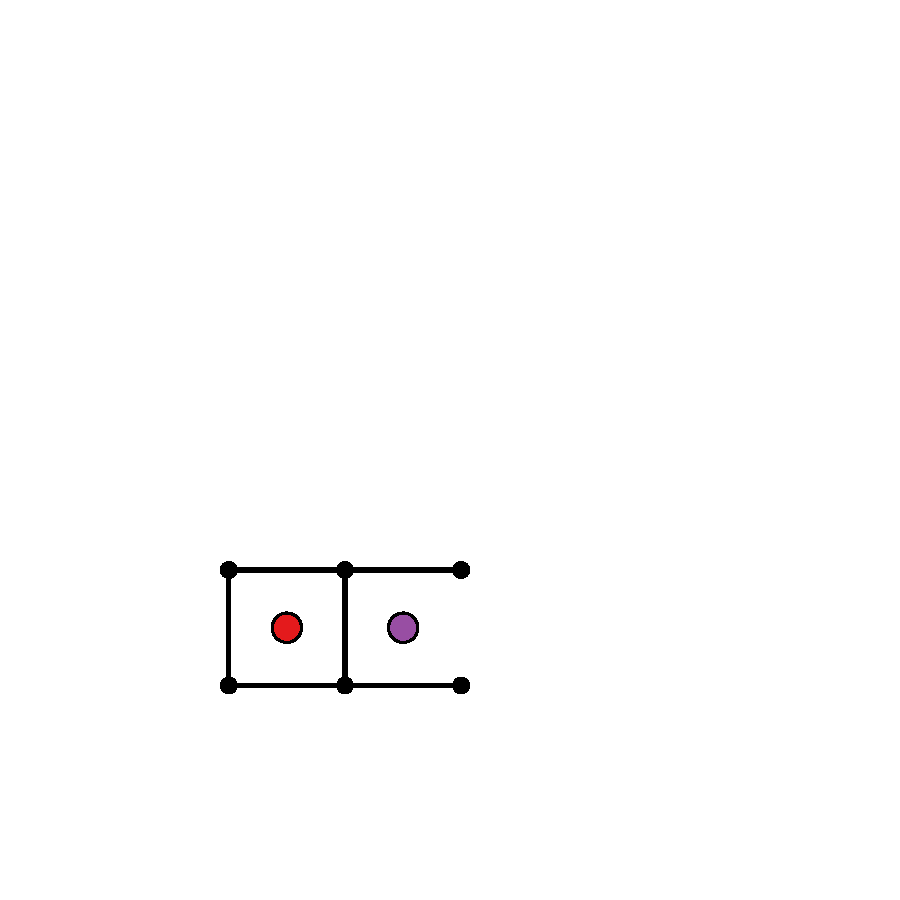
\includegraphics[height=1.2cm]{./figures/procrystals/2x1_2.pdf}
         \caption{}
         \label{fig:et2x1_2}
     \end{subfigure}
     \hfill
    \begin{subfigure}[b]{0.19\textwidth}
         \centering
         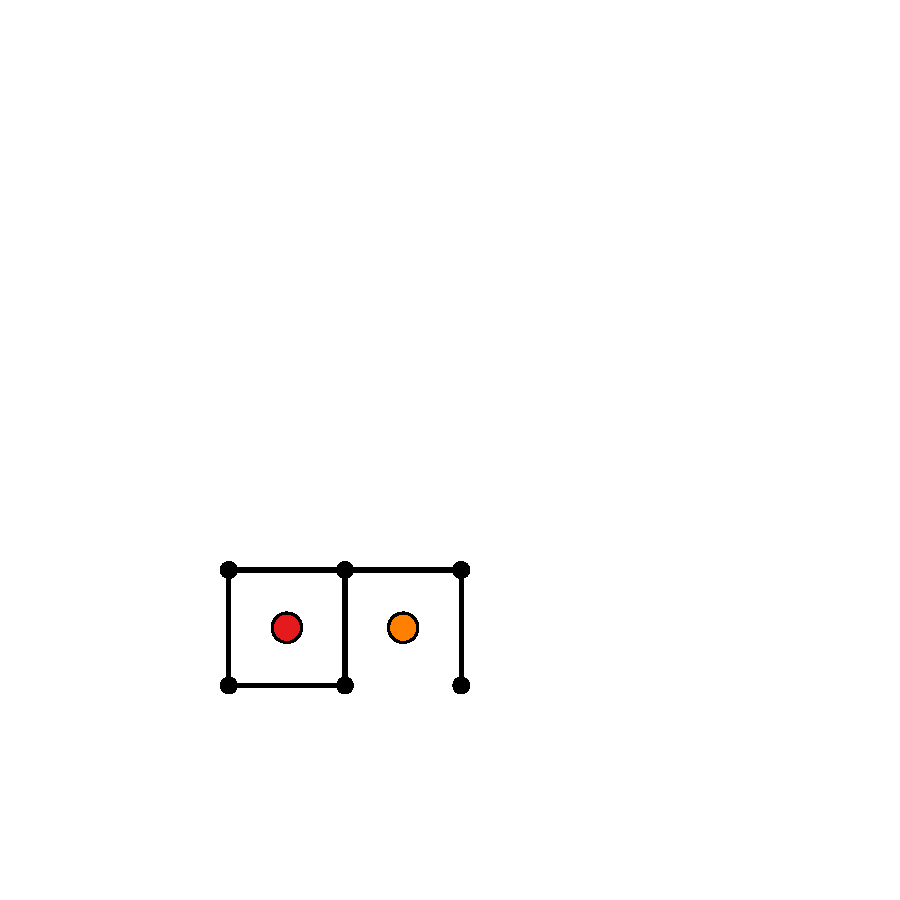
\includegraphics[height=1.2cm]{./figures/procrystals/2x1_3.pdf}
         \caption{}
         \label{fig:et2x1_3}
     \end{subfigure}
     \hfill
    \begin{subfigure}[b]{0.19\textwidth}
         \centering
         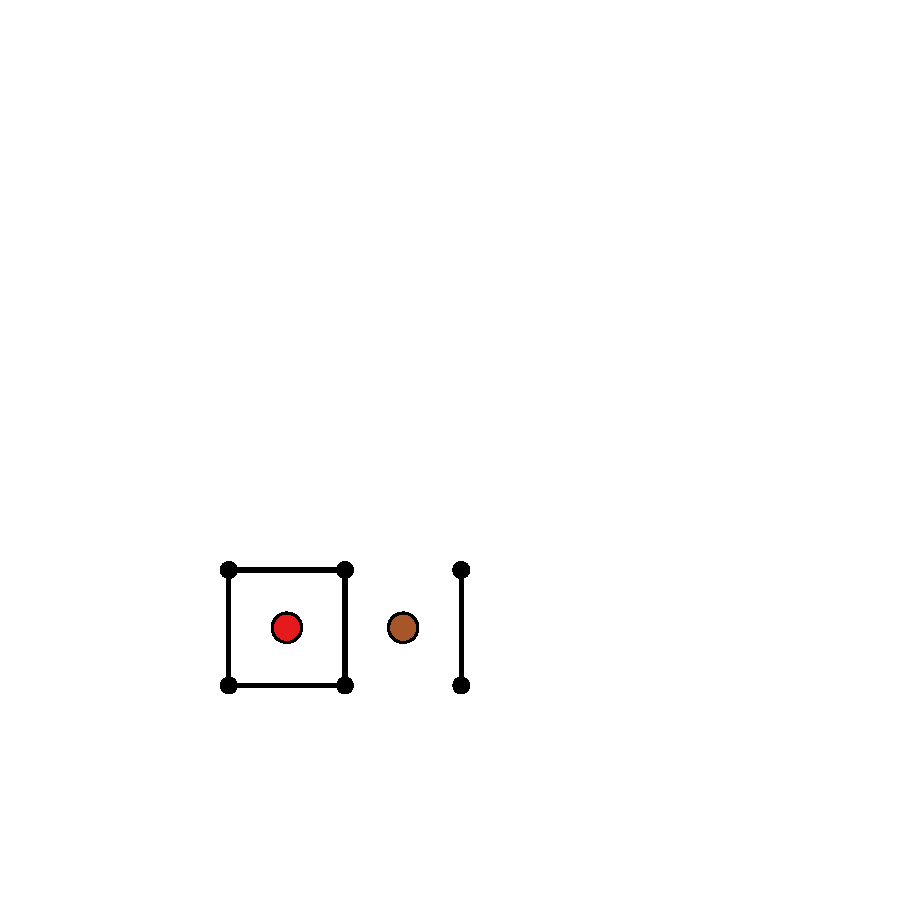
\includegraphics[height=1.2cm]{./figures/procrystals/2x1_4.pdf}
         \caption{}
         \label{fig:et2x1_4}
     \end{subfigure}
     \hfill
	\vspace{0.5cm}     

	\begin{subfigure}[b]{0.19\textwidth}
         \centering
         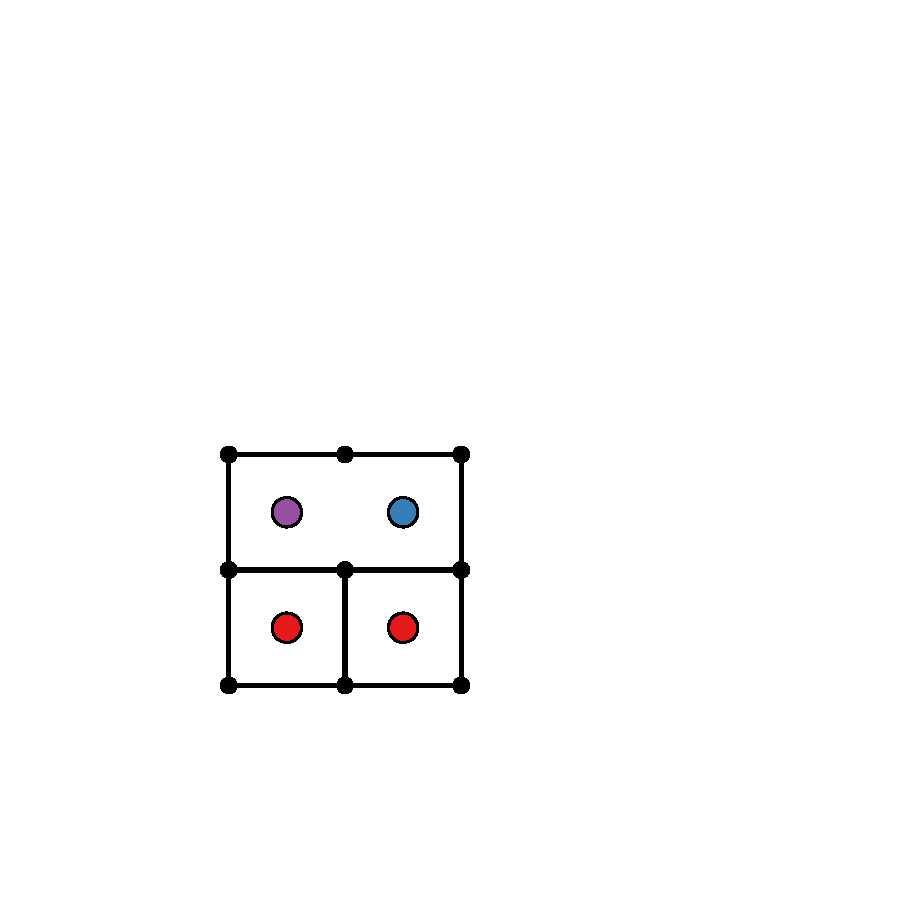
\includegraphics[height=2.2cm]{./figures/procrystals/2x2_10.pdf}
         \caption{}
         \label{fig:et2x2_0}
     \end{subfigure}
     \hfill          
     \begin{subfigure}[b]{0.19\textwidth}
         \centering
         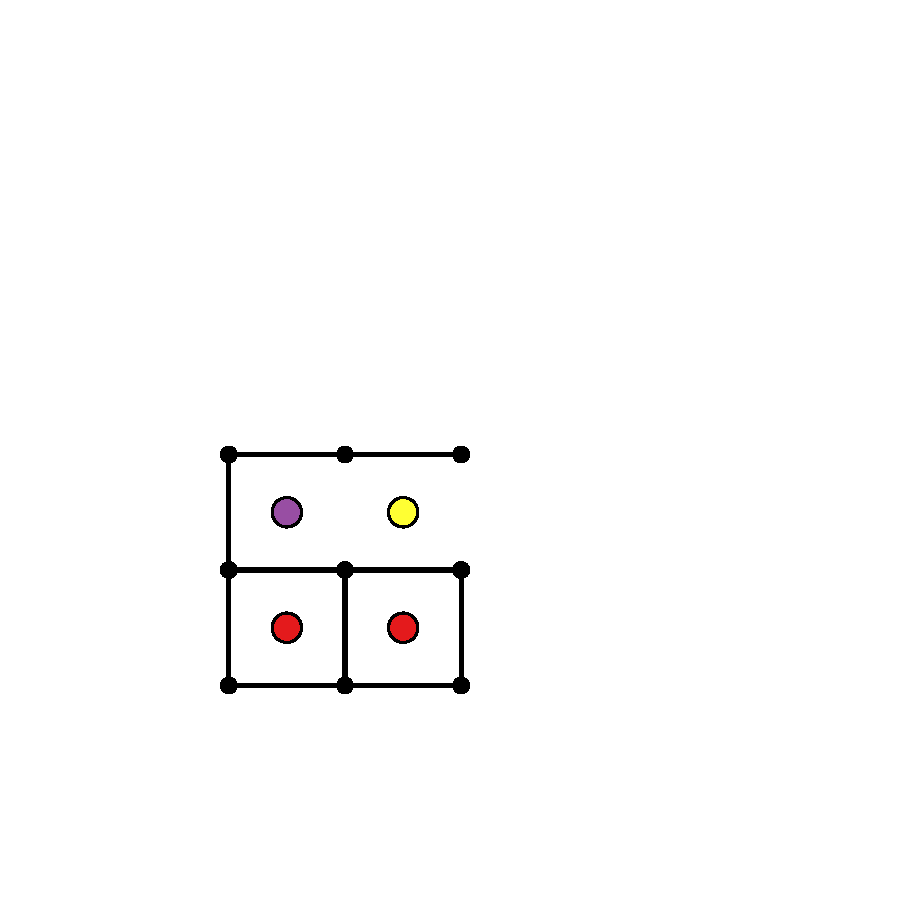
\includegraphics[height=2.2cm]{./figures/procrystals/2x2_11.pdf}
         \caption{}
         \label{fig:et2x2_1}
     \end{subfigure}
     \hfill
     \begin{subfigure}[b]{0.19\textwidth}
         \centering
         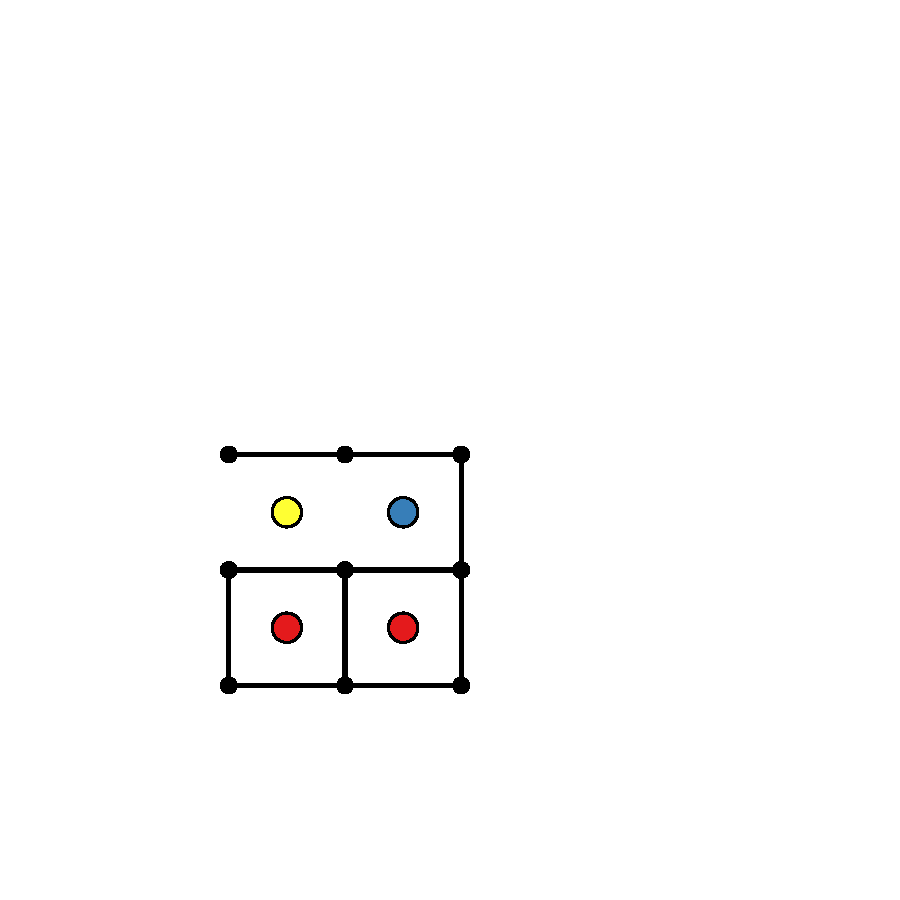
\includegraphics[height=2.2cm]{./figures/procrystals/2x2_15.pdf}
         \caption{}
         \label{fig:et2x2_2}
     \end{subfigure}
     \hfill
     \begin{subfigure}[b]{0.19\textwidth}
         \centering
         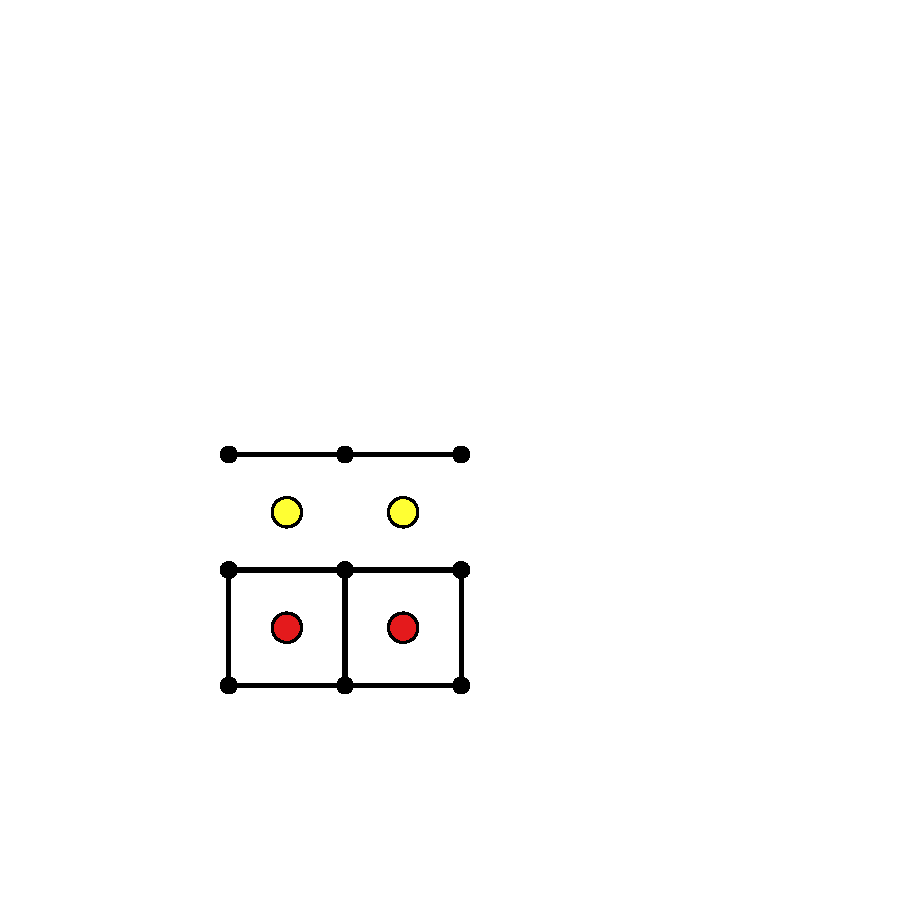
\includegraphics[height=2.2cm]{./figures/procrystals/2x2_16.pdf}
         \caption{}
         \label{fig:et2x2_3}
     \end{subfigure}
     \hfill
	
	\vspace{0.5cm}    
    
     \begin{subfigure}[b]{0.19\textwidth}
         \centering
         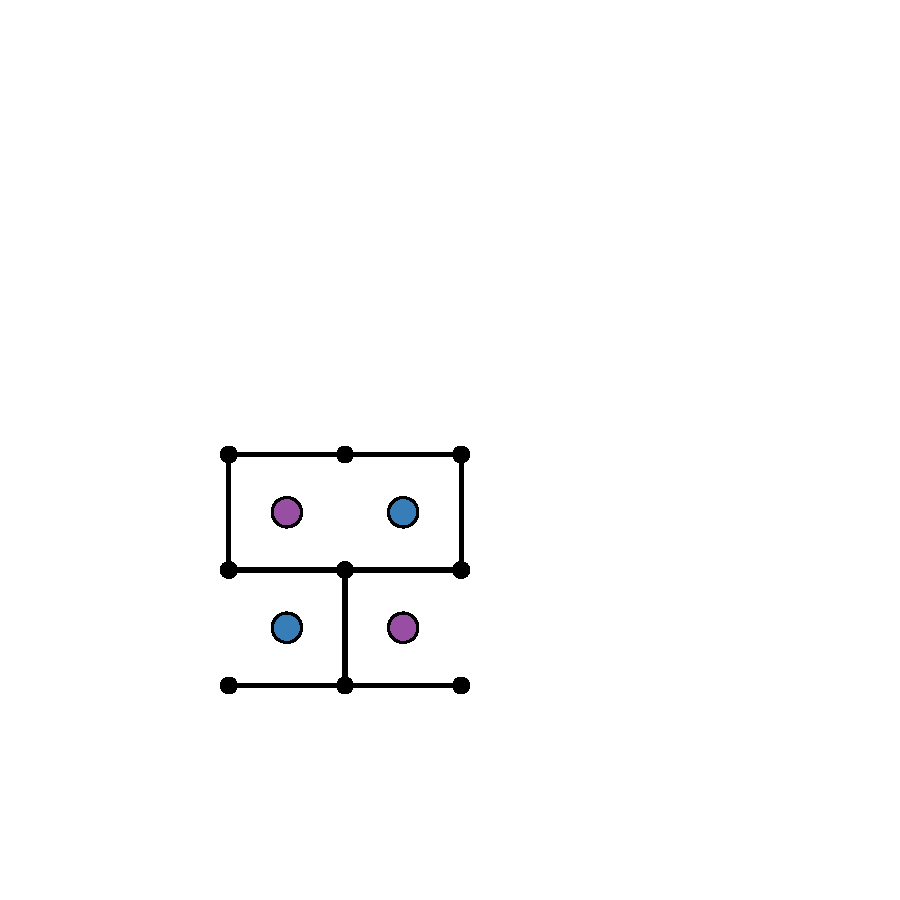
\includegraphics[height=2.2cm]{./figures/procrystals/2x2_0p.pdf}
         \caption{}
         \label{fig:et2x2p_0}
     \end{subfigure}
     \hfill
      \begin{subfigure}[b]{0.19\textwidth}
         \centering
         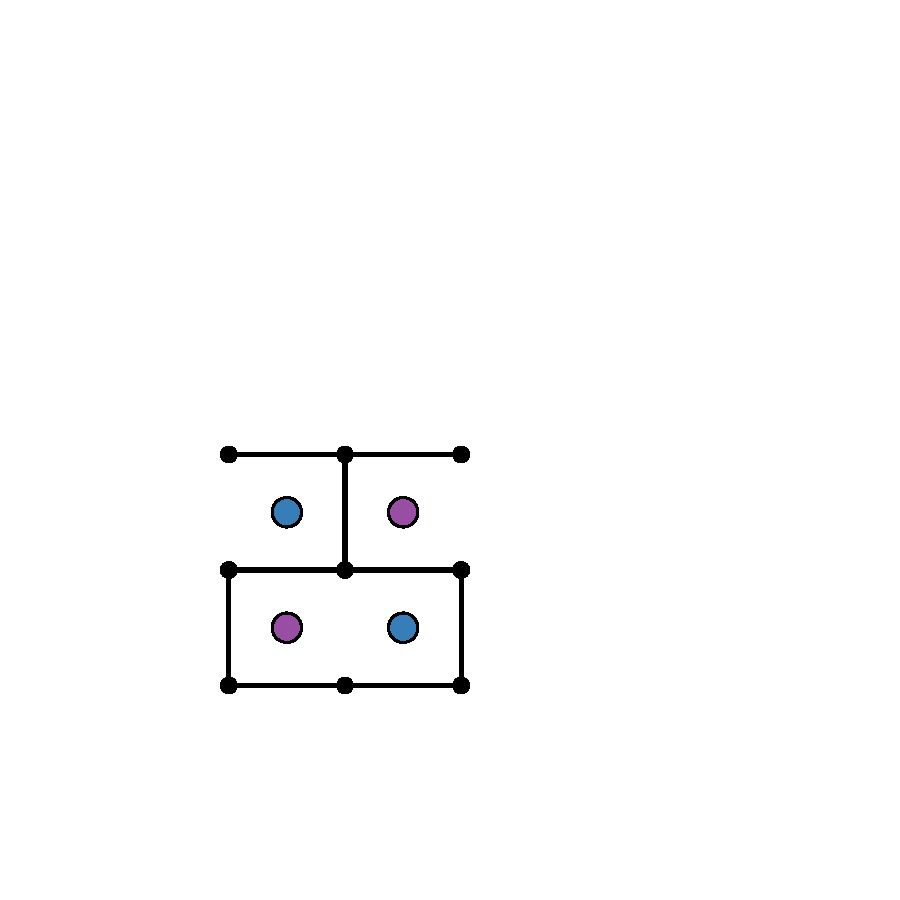
\includegraphics[height=2.2cm]{./figures/procrystals/2x2_2p.pdf}
         \caption{}
         \label{fig:et2x2p_1}
     \end{subfigure}
     \hfill
      \begin{subfigure}[b]{0.19\textwidth}
         \centering
         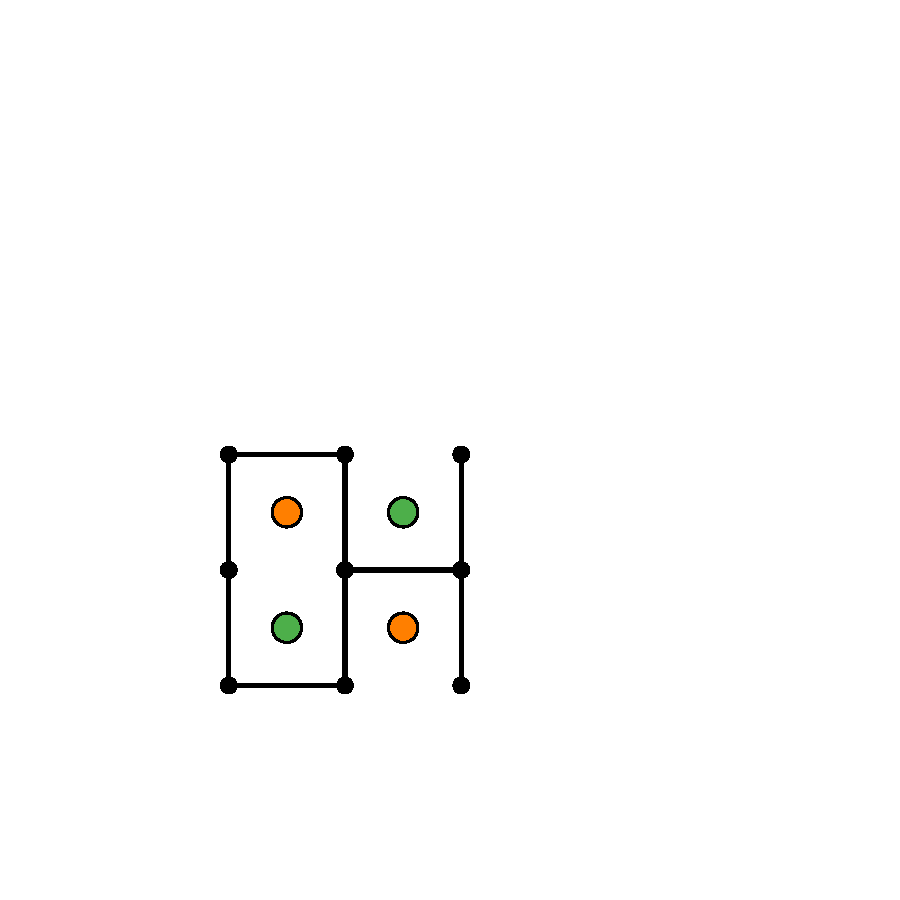
\includegraphics[height=2.2cm]{./figures/procrystals/2x2_1p.pdf}
         \caption{}
         \label{fig:et2x2p_2}
     \end{subfigure}
     \hfill
      \begin{subfigure}[b]{0.19\textwidth}
         \centering
         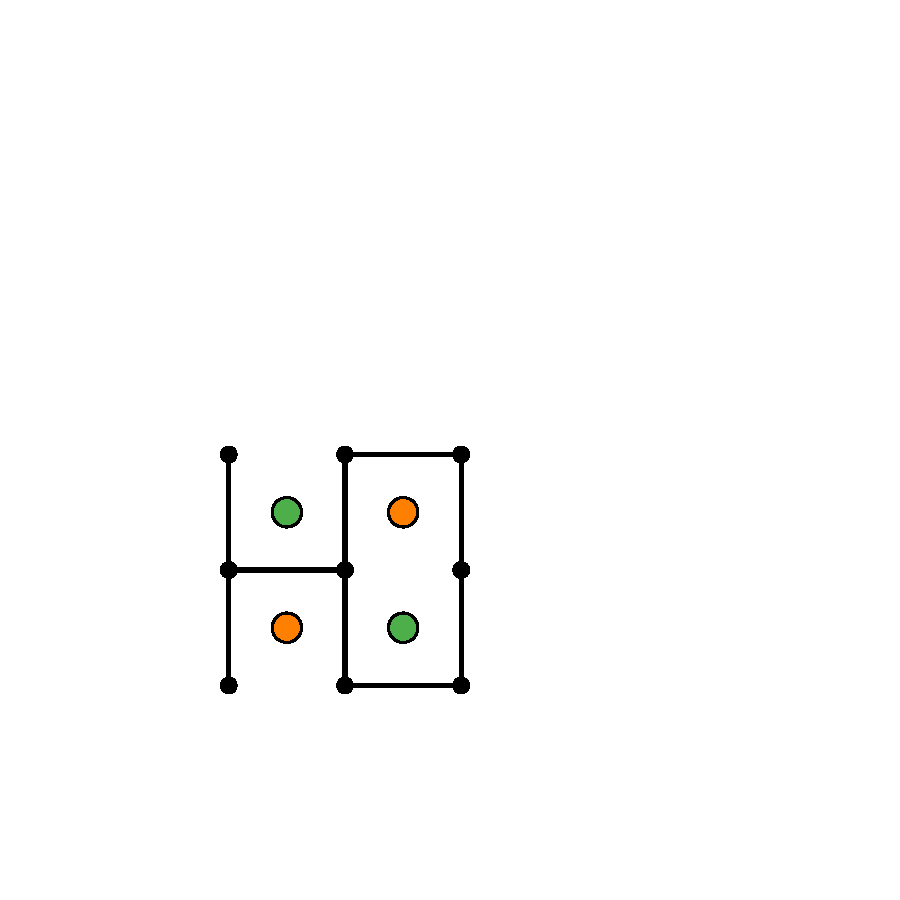
\includegraphics[height=2.2cm]{./figures/procrystals/2x2_3p.pdf}
         \caption{}
         \label{fig:et2x2p_3}
     \end{subfigure}
     \hfill
    
     \caption{Illustration of the process of exact tiling. Panels (a)\--(g) give the 7 fundamental $1\times 1$ environments for a square in the \pro{4}{3}square lattice (individually coloured with a central circle, merely intended a guide for the eye). These can be combined to give $2\times 1$ tiles, the 5 acceptable tiles using (a) shown in panels (h)\--(l). The process can be repeated to build up larger tiles such as the $2\times 2$ tiles in (m)\--(p). Finally the periodic tiles can be identified, the 4 only $2\times 2$ cases given in (q)\--(t).}
     \label{fig:exacttiling}
\end{figure}

It should be clear that this process of combining smaller tiles to form larger tiles can be continued \adinfinitum{}, producing tiles of arbitrary dimension $m\times n$.
This method is vastly more efficient than a brute force search to obtain the same structures, where notionally each ``T'' can adopt 4 positions leading to $4^{m\times n}$ possible configurations - only a fraction of which satisfy the bonding requirements.
The key to the exact tiling method is only to retain units in which the bulk nodes (\ie{} those not on the perimeter) are all 3\--coordinate, thus dramatically reducing the search space.
In order to find the periodic procrystals for a $m\times n$ lattice, one then only has to check for units which can tessellate with $3$\--coordination on the perimeter nodes.
For the $2\times 2$ lattice, only $4 / 84$ of the tiles conform to this rule, shown in figures \ref{fig:et2x2p_0}\--\ref{fig:et2x2p_3}.
It is further evident that these $4$ configurations are all in fact symmetry related, and that the only unique solution is in fact the hexagonal tiling.

The ability to leverage symmetry to reduce the search space further is important when looking at larger lattices. 
This can be achieved by identifying and discarding tiles that are symmetrically equivalent.
Care must be taken however to still form larger tiles by adding the original degenerate set to the reduced set, to avoid losing solutions.
A final improvement can be to check for ``half\--periodicity'' when forming $2m\times n$ tiles from $m\times n$ tiles. 
In this case any units which are not periodic in the fixed dimension can also be discarded before combination takes place.

\begin{table}[bt]
	\centering
     \caption{Performance of the exact tiling algorithm. For each lattice dimension the number of aperiodic, periodic and symmetrically unique periodic tiles are listed. The search space can be found by squaring the number of aperiodic tiles of the previous tile size. }
     \label{tab:exacttiling}
     \begin{tabular}{cccc}
     \toprule
     Lattice & Aperiodic & Periodic & Unique \\
     \midrule
	 $2\times 2$ & 84 & 4 & 1 \\
	 $2\times 4$ & 1,536 & 16 & 4 \\	
	 $2\times 6$ & 27,572 & 64 & 8 \\	
	 %$2\times 8$ & 493,220 & 256 & 18 \\	
	 $4\times 4$ & 87,264 & 204 & 9 \\
	 $4\times 6$ & 4,9147,56 & 2,368 & 70  \\
	 $6\times 6$ & $-$ & 81,736 & 440  \\
     \bottomrule
     \end{tabular}
\end{table}

The application of all the optimisations discussed above serve to make the exact tiling algorithm tractable for a small lattices.
Table \ref{tab:exacttiling} details the performance of the algorithm.
Taking even the $4\times 4$ lattice as an example, a na\"ive search algorithm would require $4^{16}\sim 4\times10^9$ iterations compared to the $1536^2\sim 2\times10^6$ for the exact tiling algorithm.
The difference for the $6\times 6$ lattice becomes even more marked, spanning some 8 orders of magnitude.
However, it is still fighting against the forces of exponential scaling and despite all these improvements in performance, the exact tiling algorithm remains severely limited. 
Table \ref{tab:exacttiling} highlights the enormity of the full configurational space and how small a proportion the procrystal solutions are of the total.
In order to find all the solutions for larger lattices, a more sophisticated algorithm would be required, although it is hard to see how the hurdle of scaling could be easily overcome.

\subsection{Monte Carlo Algorithm}

To generate procrystals for larger lattice dimensions, a method is required that can quickly search configurational space and find representative samples.
As with much of the work in this thesis, this is achieved by utilising a \mc{} algorithm.
The algorithm in question has been developed to produce \pro{c^\prime}{c}lattices of arbitrary size.
It is a zero\--temperature \mc{} algorithm which proceeds as follows:
\begin{enumerate}
	\item Initialise the required $c^\prime$\--coordinate periodic lattice from figure \ref{fig:symlat} and assign each node $c$ bonds in a random orientation. This will introduce a number of dangling bonds into the configuration.
	\item Select a node at random and change the orientation of the bonds.
	\item If the number of dangling bonds is less than or equal to the number in the previous configuration update the configuration; otherwise revert to the previous structure.
	\item Repeat steps 2 and 3 until all dangling bonds have been removed and all node coordinations are satisfied.
	The final lattice is then in the procrystalline state.
\end{enumerate}
This process is demonstrated for an $8\times 8$ \pro{4}{3}square lattice in figure \ref{fig:promc}.
One aspect of note is that as removing the dangling bonds often requires a correlated motion, it becomes increasingly difficult to remove defects as they reduce in number.
Furthermore the structure obtained with a small number of dangling bonds can be quite different to the final procrystalline network as a consequence of the required reorganisation.

This method can be thought of as a simplified version of a site adsorption model, where molecules adsorb to specific sites on an underlying lattice and interact with varying directional potentials \cite{Gorbunov2017,Nieckarz2018,Buzano2004}.
The difference is that here the potential model is binary and the aim of the method is to generate a fully coordinate, defect\--free ``ground state'' procrystalline lattice.
One could in principle introduce a Metropolis type criterion into step 3 (with the the energy difference reflecting the change in number of dangling bonds) and hence accepting a proportion of ``uphill'' moves.
However, the zero\--temperature version is found to converge very well, as there is sufficient flexibility through moves which merely conserve the number of dangling bonds for a global minimum to be reached.
In addition, the temperature parameter was not found to appreciably affect the overall properties of the resulting realisations.

\begin{figure}[bt]
     \centering
     
     \begin{subfigure}[b]{0.3\textwidth}
         \centering
         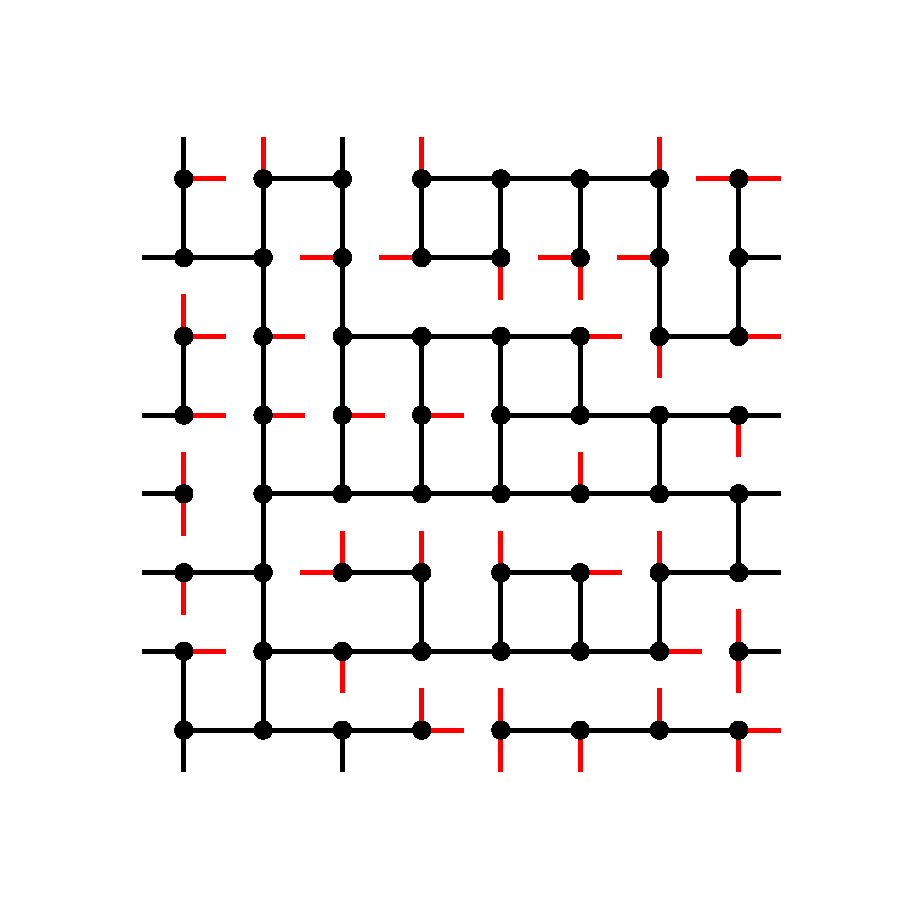
\includegraphics[width=\textwidth]{./figures/procrystals/pro_mc_1.pdf}
         \caption{Initial random lattice.}
         \label{fig:promca}
     \end{subfigure}
     \hfill
     \begin{subfigure}[b]{0.3\textwidth}
         \centering
         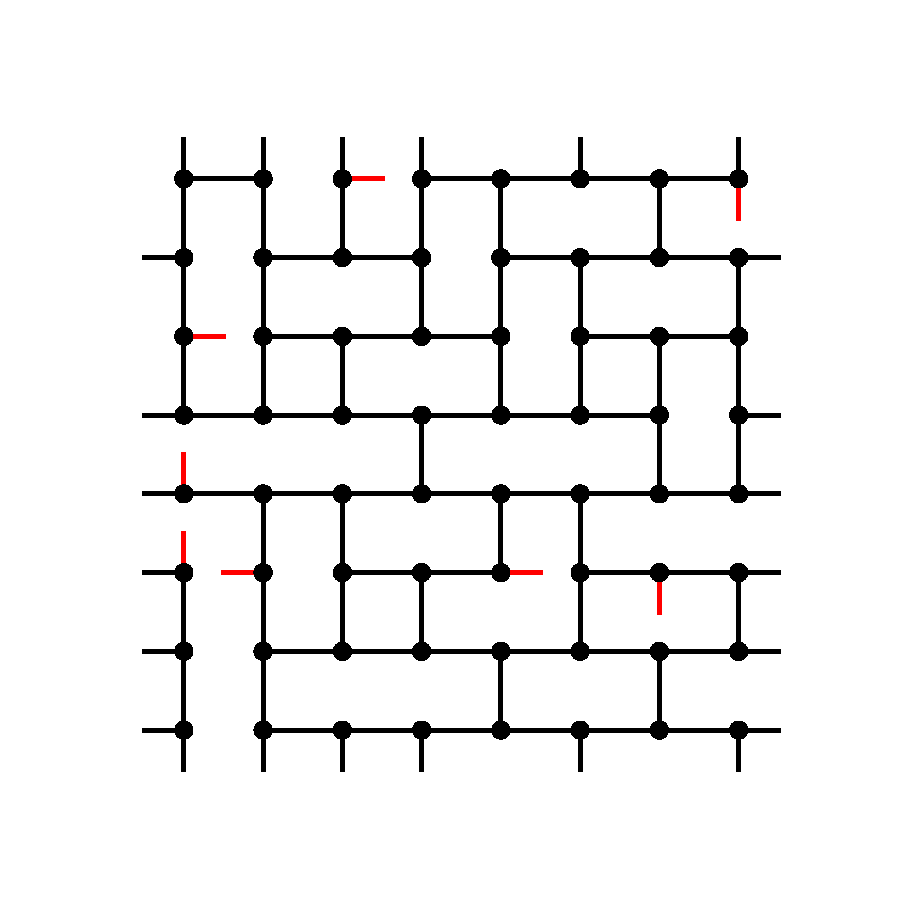
\includegraphics[width=\textwidth]{./figures/procrystals/pro_mc_3.pdf}
         \caption{Partial convergence.}
         \label{fig:promcb}
     \end{subfigure}
     \hfill
     \begin{subfigure}[b]{0.3\textwidth}
         \centering
         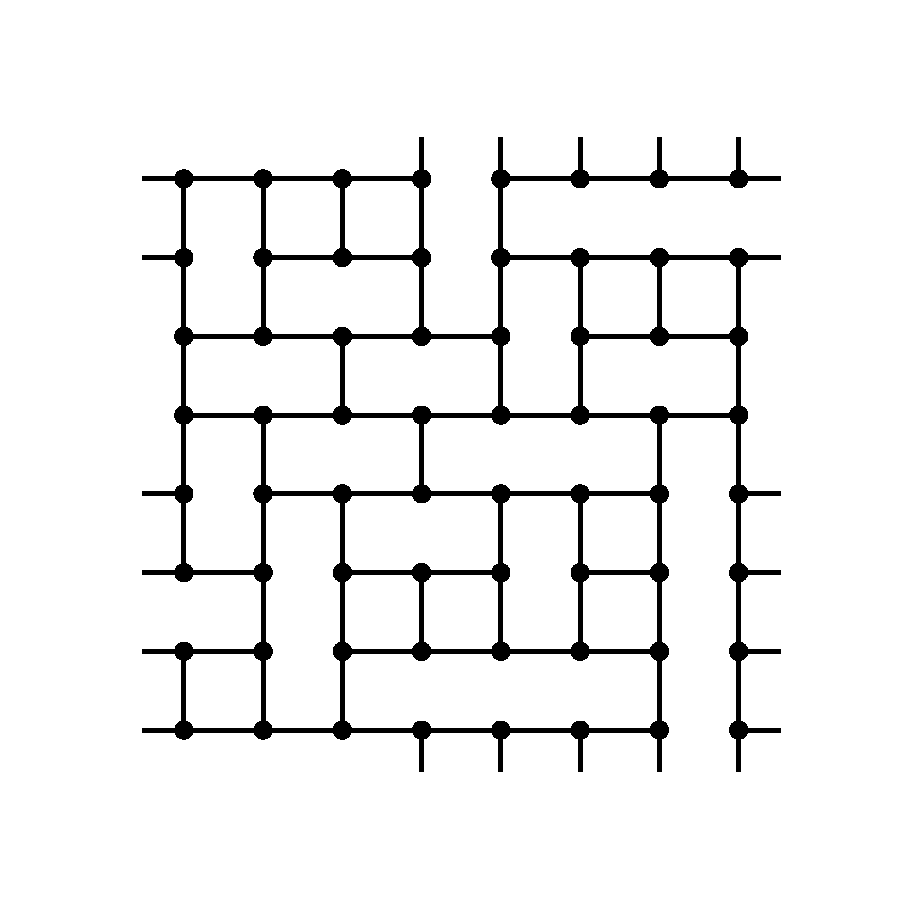
\includegraphics[width=\textwidth]{./figures/procrystals/pro_mc_4.pdf}
         \caption{Procrystalline lattice.}
         \label{fig:promcc}
     \end{subfigure}
     \hfill
     
     \caption{Stages in the \mc{} search for \pro{4}{3}square procrystalline lattices. Panel (a) gives the initial lattice where each node has 3 bonds in random orientations, panel (b) a snapshot during the search where dangling bonds are being removed and panel (c) the final lattice. Satisfied bonds are coloured black and dangling bonds red.}
     \label{fig:promc}
\end{figure}

\section{Structure of 3\--Coordinate Procrystals}
\label{s:pro3}

The bulk of the investigation in this chapter will focus on \pro{c^\prime}{3}procrystalline lattices. 
As stated before, this is because such systems are most prevalent in nature and draw parallels with previous work. 
To study the ring structure of these procrystals, the \mc{} method detailed in \davidnote{ref} was used to generate configurations for each of the five underlying lattice types, with number of nodes, $V$, in the lattice scaled to explore system size effects.
For each set of parameters some $100,000$ periodic procrystalline lattices were generated.
A visualisation of an example configuration based on each parent lattice type is given in figure \ref{fig:pro3} for reference. 
These configurations highlight some important features of the specific procrystalline lattices which will will be a useful for the coming discussions.

\begin{itemize}
	\item $\mathbf{4,3-}$\textbf{square}: only contains even\--membered rings in the set $k\in\left\{4,6,8\cdots\right\}$. The results from the lack of ``cross'' bonds (acting between opposite corners of a square). Rings must be linear as any ``L''\--shapes would require stabilisation of a $2$\--coordinate site. 
	\item $\mathbf{4,3-}$\textbf{trihexagonal}: is yet more constrained, containing only rings in the set $k=\left\{3,6,7,8,9\right\}$. Each ``large'' ring ($k>3$) is surrounded by $k-6$ triangles.
	\item $\mathbf{5,3-}$\textbf{elongated\--triangular}: difference between underlying and procrystalline lattice is now $2$ and the full ring size range is accessible $k\in\left\{3,4,5\dots\right\}$.
	\item $\mathbf{5,3-}$\textbf{snub\--square}: as above.
	\item $\mathbf{6,3-}$\textbf{triangular}: difference between underlying and procrystalline lattice is now $3$ and again $k\in\left\{3,4,5\dots\right\}$.	
\end{itemize}

\begin{figure}[bt]
     \centering
     
     \begin{subfigure}[b]{0.45\textwidth}
         \centering
         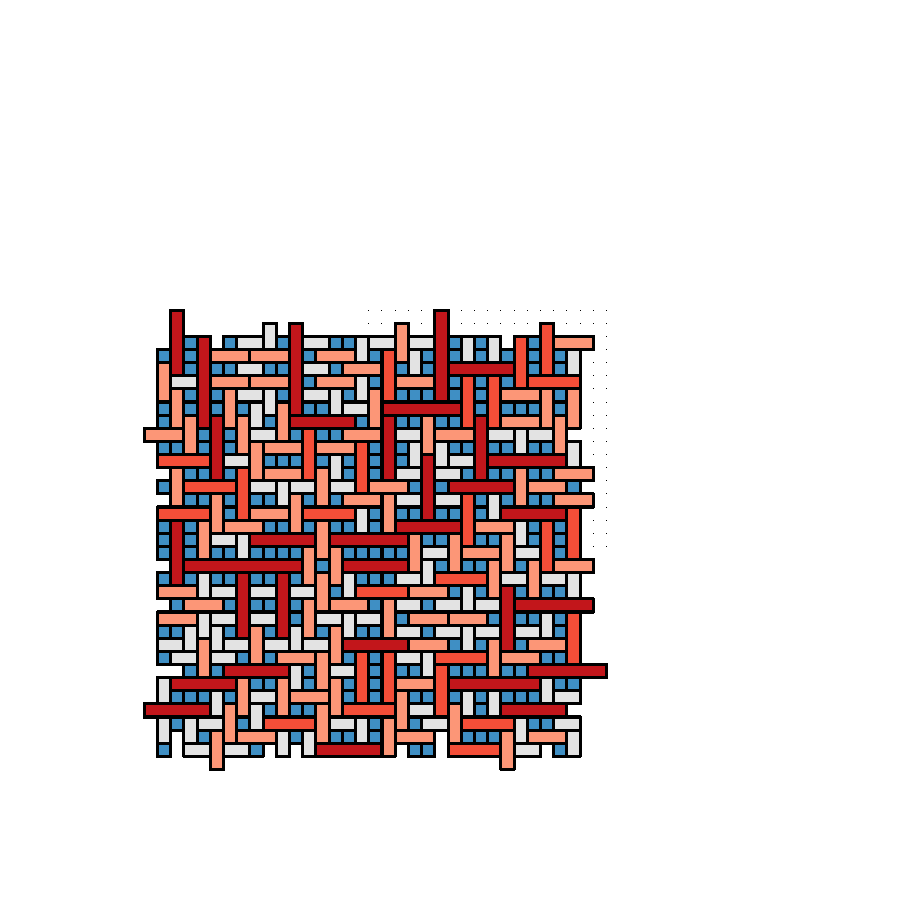
\includegraphics[height=4.5cm]{./figures/procrystals/pro_sq3.pdf}
         \caption{\pro{4}{3}square}
         \label{fig:pro3a}
     \end{subfigure}
      \begin{subfigure}[b]{0.45\textwidth}
         \centering
         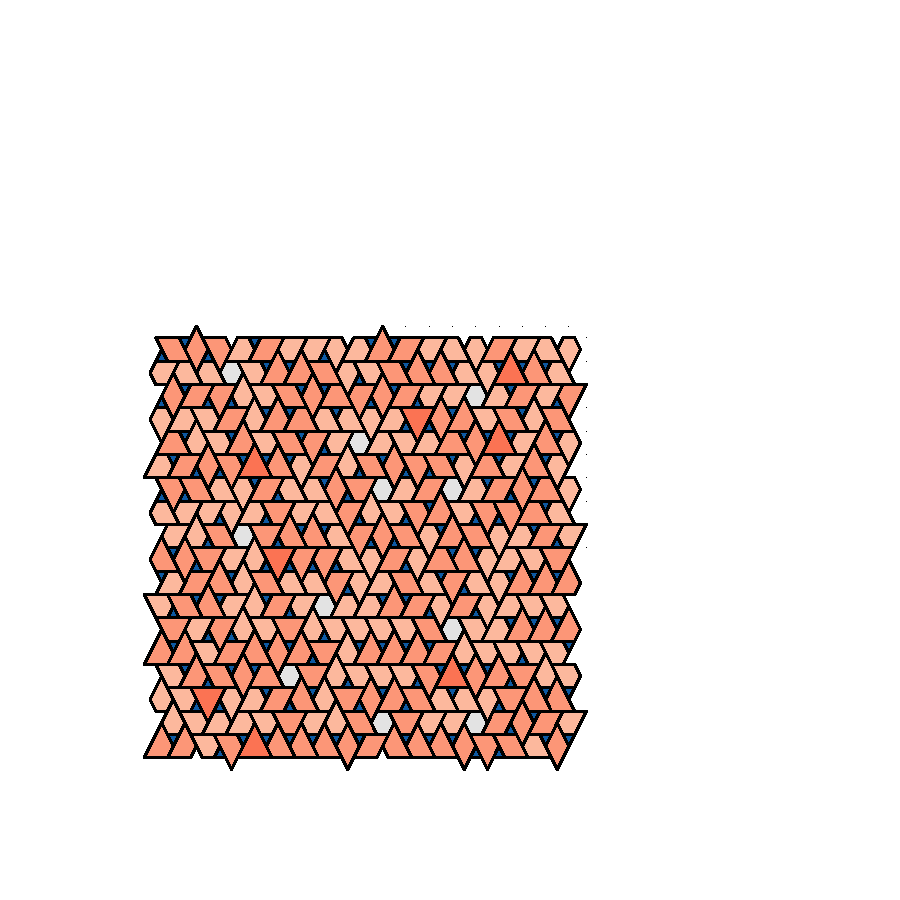
\includegraphics[height=4.5cm]{./figures/procrystals/pro_trihex3.pdf}
         \caption{\pro{4}{3}trihexagonal}
         \label{fig:pro3b}
     \end{subfigure}
     \hfill
     	
     \vspace{0.5cm}
     \begin{subfigure}[b]{0.45\textwidth}
         \centering
         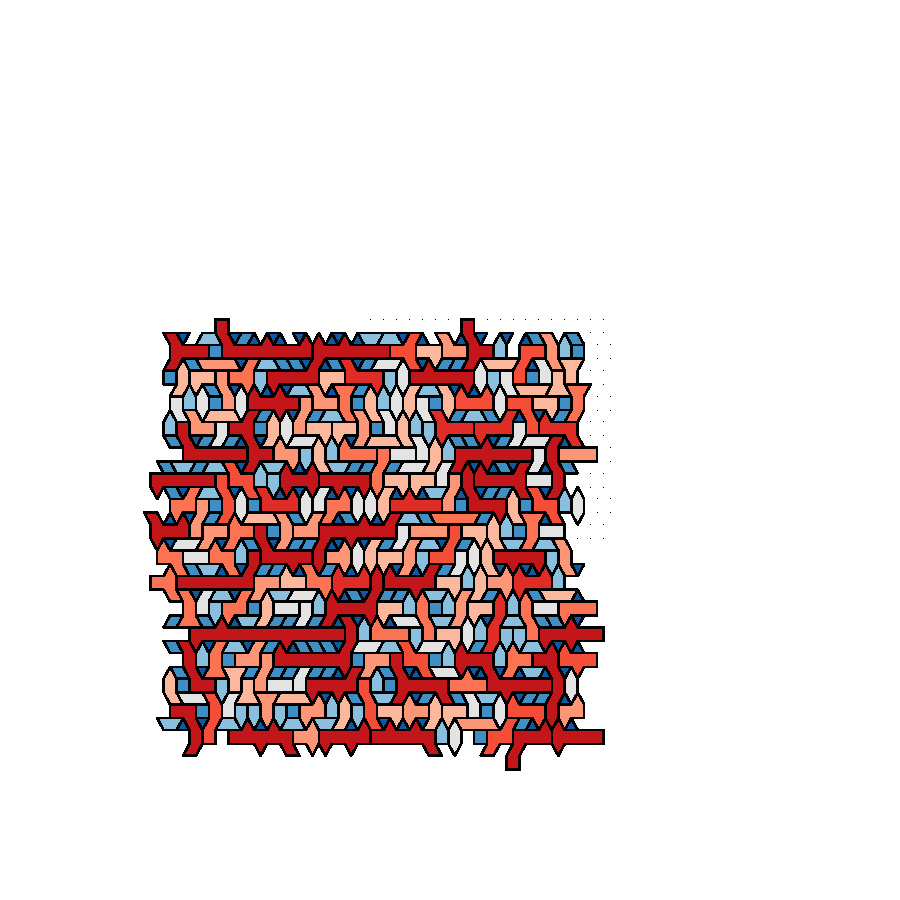
\includegraphics[height=4.5cm]{./figures/procrystals/pro_elong3.pdf}
         \caption{\pro{5}{3}elongated\--triangular}
         \label{fig:pro3c}
     \end{subfigure}
     \begin{subfigure}[b]{0.45\textwidth}
         \centering
         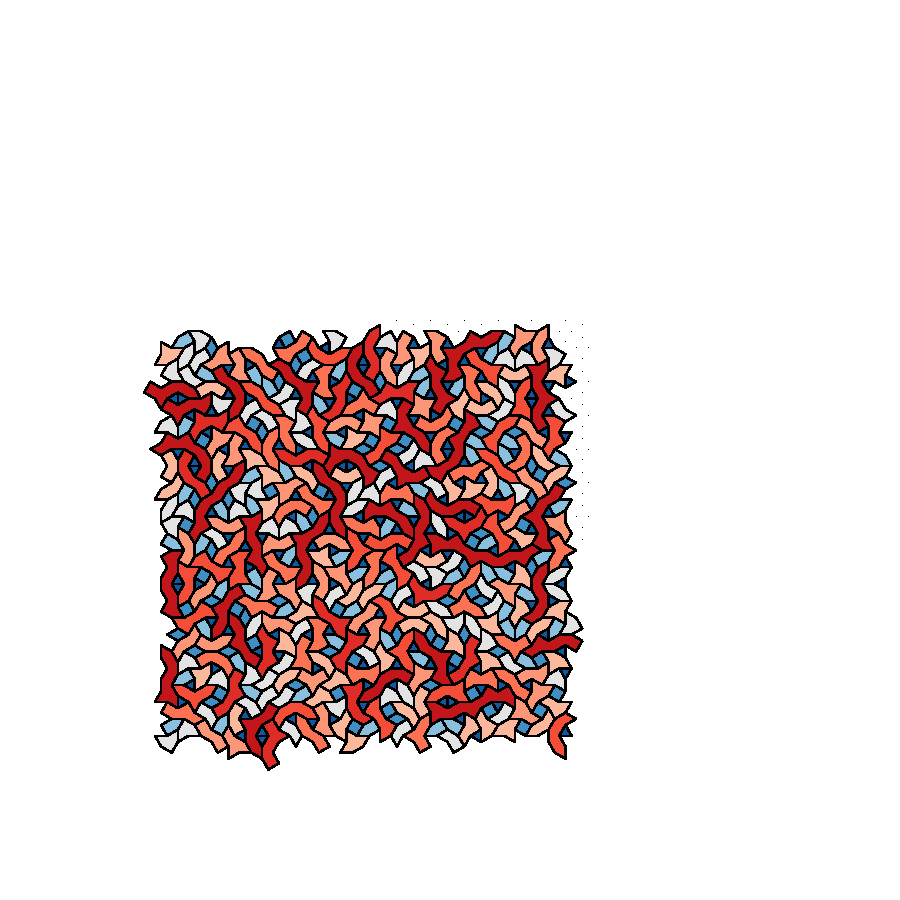
\includegraphics[height=4.5cm]{./figures/procrystals/pro_snub3.pdf}
         \caption{\pro{5}{3}snub\--square}
         \label{fig:pro3d}
     \end{subfigure}
     \hfill
     
     \vspace{0.5cm}     
     \begin{subfigure}[b]{0.45\textwidth}
         \centering
         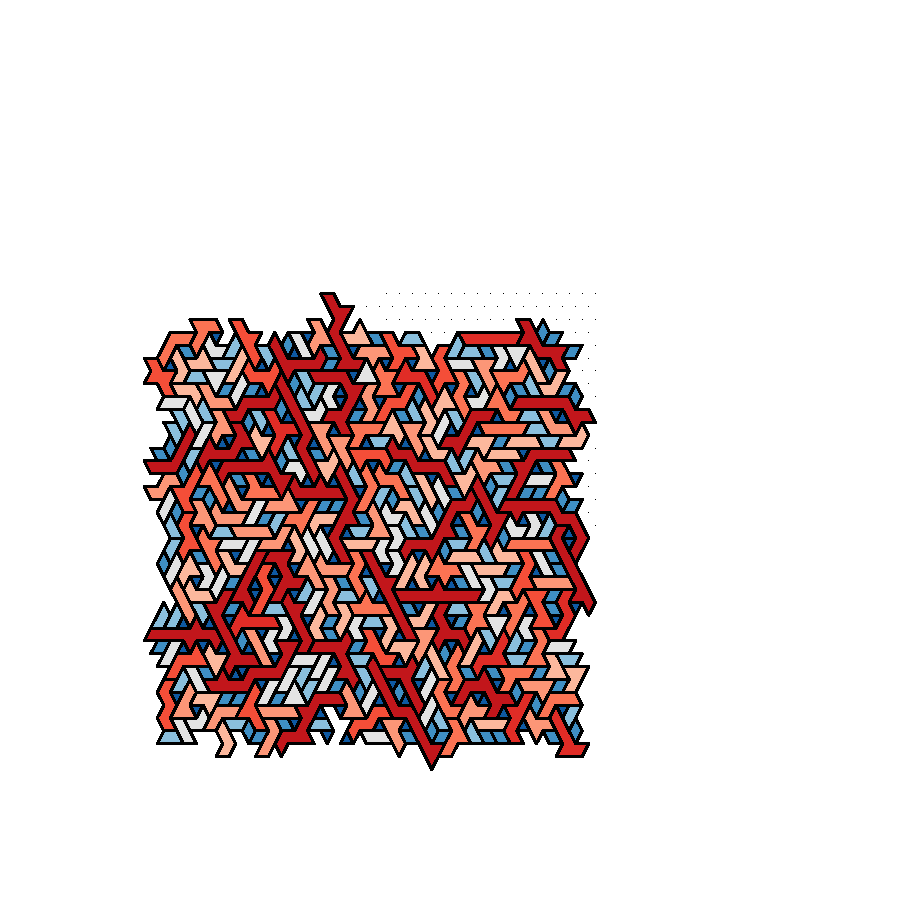
\includegraphics[height=4.5cm]{./figures/procrystals/pro_tri3.pdf}
         \caption{\pro{6}{3}triangular}
         \label{fig:pro3e}
     \end{subfigure}
     \hfill
    
     \caption{Visualisations of 3\--coordinate procrystals based on the 5 different parent lattices (as indicated in panel captions).}
     \label{fig:pro3}
\end{figure}

Importantly, these 3\--coordinate procrystals will be compared and contrasted with two other states.
The first are networks generated from bond switching at infinite temperature \davidnote{link}, which is in effect a method for producing continuous random networks (CRNs) \ie{} a fully amorphous state.
The second are series of crystalline motifs of the form $8-6^i-5^2$ and $8-6^i-4$ for $0\leq i\leq3$ (the nomenclature indicating the number of each ring size in the unit cell) taken from Altman \etal{} \cite{Malashevich2016}.

\subsection{Ring Size Distributions}

The first structural measure that will be investigated is the ring size distribution.
These will be compared to the maximum entropy (ME) distributions given by equation \ref{eq:prome}, with the accessible $k$\--range for each procrystal outlined in section \ref{s:pro3} above. 
For instance, given the \pro{4}{3}square lattice one might expect it to follow a maximum entropy ring distribution of the form:
\begin{equation}
	\pme_k = \left(\frac{1}{2}\right)^{k/2-1}\,, \qquad k\in\left\{4,6,8\cdots\right\}\,.
\end{equation}
Similarly for the lattices which can accommodate any ring size, the comparative maximum entropy distribution is:
\begin{equation}
	\pme_k = \left(\frac{1}{4}\right)\left(\frac{3}{4}\right)^{k-3}\,, \qquad k\in\left\{3,4,5\cdots\right\}\,.
\end{equation}
These purpose of these maximum entropy distributions is to highlight any discrepancies between the procrystalline systems and an equivalent random lattice.

\begin{figure}[btp]
     \centering
     
     \begin{subfigure}[b]{0.40\textwidth}
         \centering
         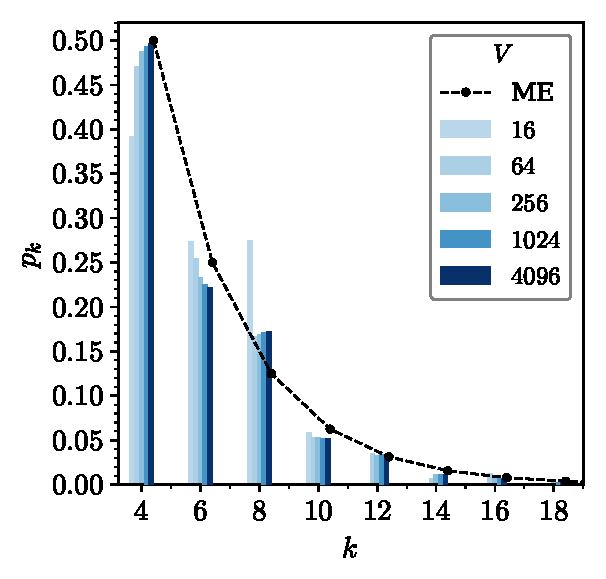
\includegraphics[width=\textwidth]{./figures/procrystals/sq3_pk.pdf}
         \caption{\pro{4}{3}square}
         \label{fig:pro3pka}
     \end{subfigure}
          \hfill
      \begin{subfigure}[b]{0.40\textwidth}
         \centering
         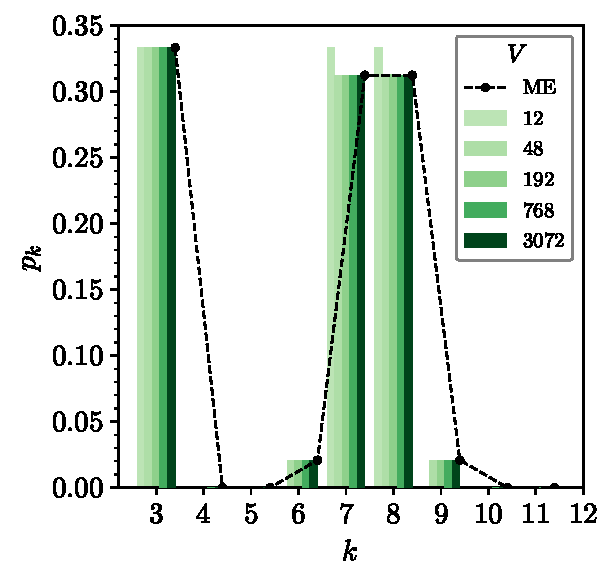
\includegraphics[width=\textwidth]{./figures/procrystals/trihex3_pk.pdf}
         \caption{\pro{4}{3}trihexagonal}
         \label{fig:pro3pkb}
     \end{subfigure}
     \hfill
     	
     \vspace{0.5cm}
     \begin{subfigure}[b]{0.40\textwidth}
         \centering
         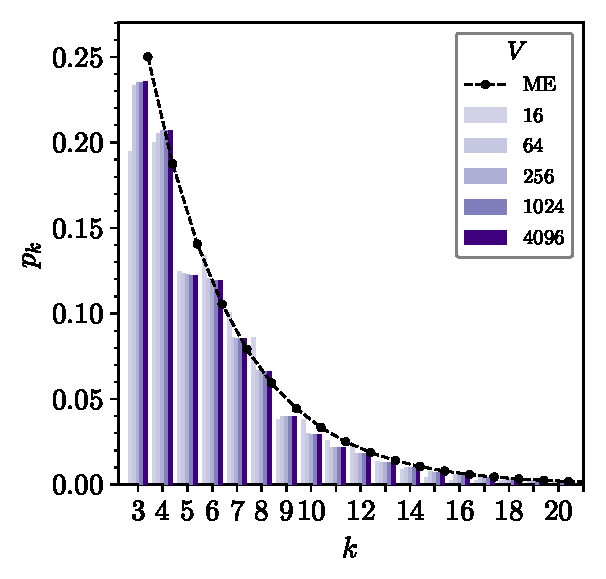
\includegraphics[width=\textwidth]{./figures/procrystals/elong3_pk.pdf}
         \caption{\pro{5}{3}elongated\--triangular}
         \label{fig:pro3pkc}
     \end{subfigure}
          \hfill
     \begin{subfigure}[b]{0.40\textwidth}
         \centering
         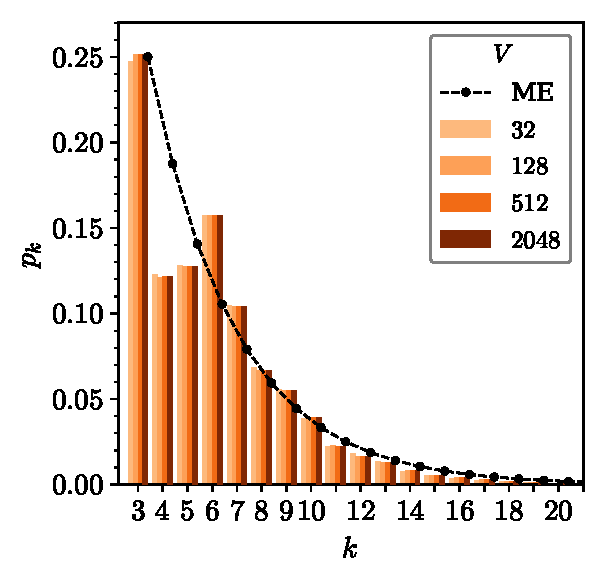
\includegraphics[width=\textwidth]{./figures/procrystals/snub3_pk.pdf}
         \caption{\pro{5}{3}snub\--square}
         \label{fig:pro3pkd}
     \end{subfigure}
     \hfill
     
     \vspace{0.5cm}
     \begin{subfigure}[b]{0.40\textwidth}
         \centering
         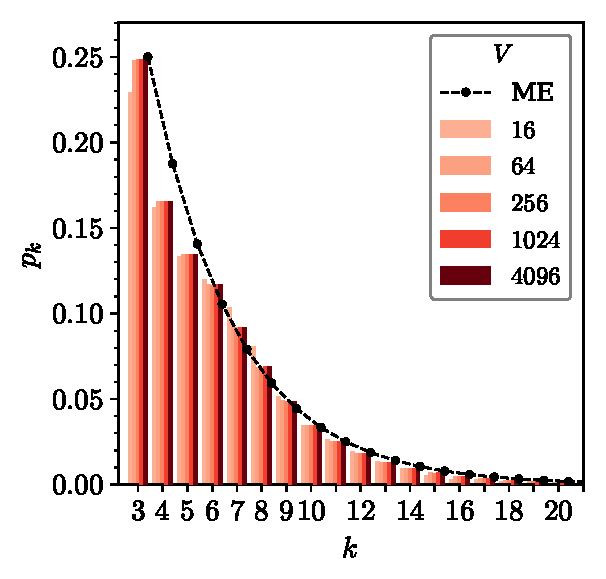
\includegraphics[width=\textwidth]{./figures/procrystals/tri3_pk.pdf}
         \caption{\pro{6}{3}triangular}
         \label{fig:pro3pke}
     \end{subfigure}
     \hfill
      \begin{subfigure}[b]{0.40\textwidth}
         \centering
         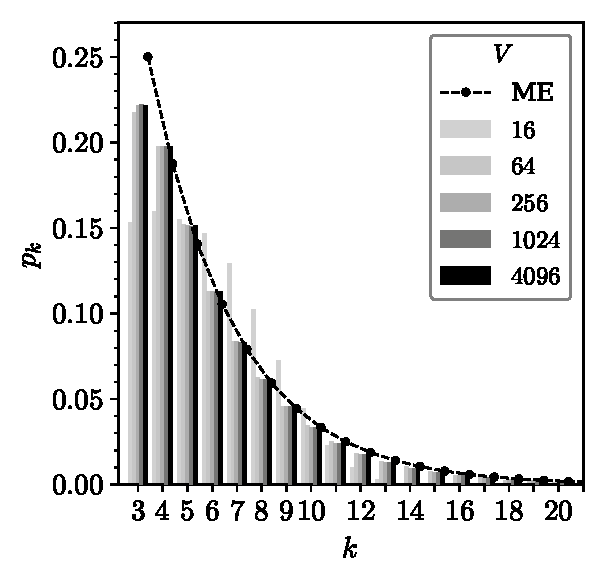
\includegraphics[width=\textwidth]{./figures/procrystals/netmc_pk.pdf}
         \caption{CRNs}
         \label{fig:pro3pkf}
     \end{subfigure}
     \hfill
    
     \caption{Ring statistics for selected 3\--coordinate procrystalline lattices (as highlighted in subfigure captions) and from bond switching (panel (f)). In  all  panels  the  points  and  dashed  lines show the respective maximum entropy (ME) solutions.  Each panel also highlights potential system size effects by showing the ring size distributions for different numbers of nodes, $V$, as highlighted in the legends.}
     \label{fig:pro3pk}
\end{figure}

Figure \ref{fig:pro3pk} shows the ring distributions generated for the five 3\--coordinate procrystalline networks shown in figure \ref{fig:prosymlat}, as well as from bond switching.
These distributions act to highlight how the different tilings impose additional, varying constraints.
As discussed above, for the \pro{4}{3}square lattice only even\--membered rings are allowed.
In addition, the $V=16$ lattice is small enough to explicitly calculate all the possible lattices using the exact tiling method.
These are depicted in figure \ref{fig:pro3pksq} and the corresponding ring statistics are provided in table \ref{tab:sqV16}.
The overall ring statistics of the $V=16$ case can then be shown to be a simple weighted average of these tilings, namely: $p_4=\frac{20}{51}$, $p_6=\frac{14}{51}$, $p_8=\frac{14}{51}$, $p_{10}=\frac{3}{51}$.
This gives confidence that the configurations generated via \mc{} are appropriately sampling the phase space.
As the lattice size increases, the ring statistics initially change markedly, before settling on values close to the ME distribution.
This demonstrates that there are important system size effects, the most obvious of which is the largest ring size which can be supported.
As only linear rings are allowed, the largest ring possible can have $k=2\left(V^{1/2}+1\right)$, which evidently limits the ring statistics.
As the lattice dimensions increase and large rings become rarer the statistics naturally converge.

\begin{figure}[bt]
     \centering
     
      \begin{subfigure}[b]{0.16\textwidth}
         \centering
         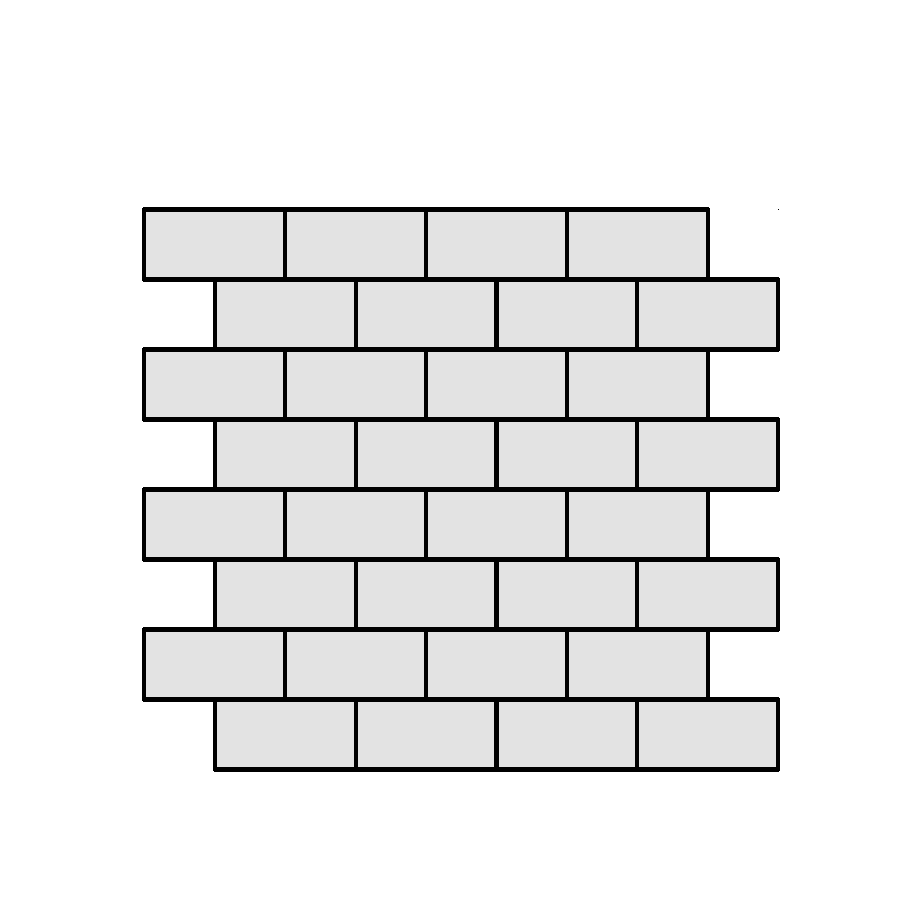
\includegraphics[width=\textwidth]{./figures/procrystals/t8.pdf}
         \caption{}
         \label{fig:pro3pksq1}
     \end{subfigure}
     \hfill
      \begin{subfigure}[b]{0.16\textwidth}
         \centering
         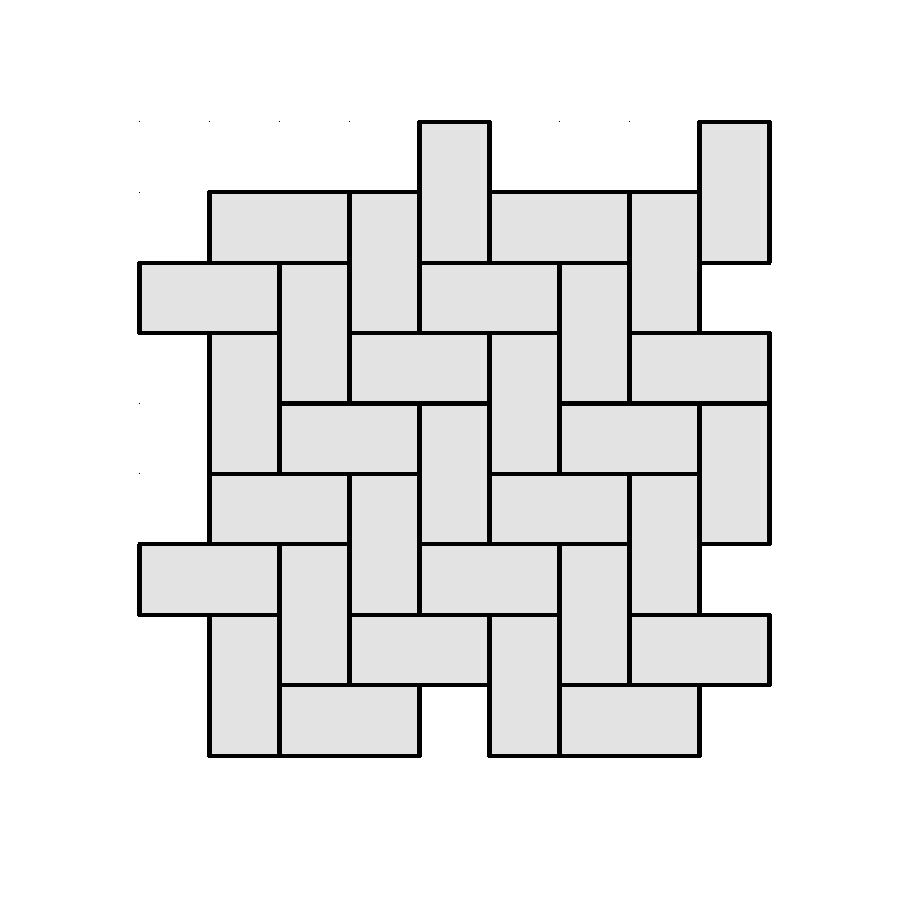
\includegraphics[width=\textwidth]{./figures/procrystals/t7.pdf}
         \caption{}
         \label{fig:pro3pksq2}
     \end{subfigure}
     \hfill
      \begin{subfigure}[b]{0.16\textwidth}
         \centering
         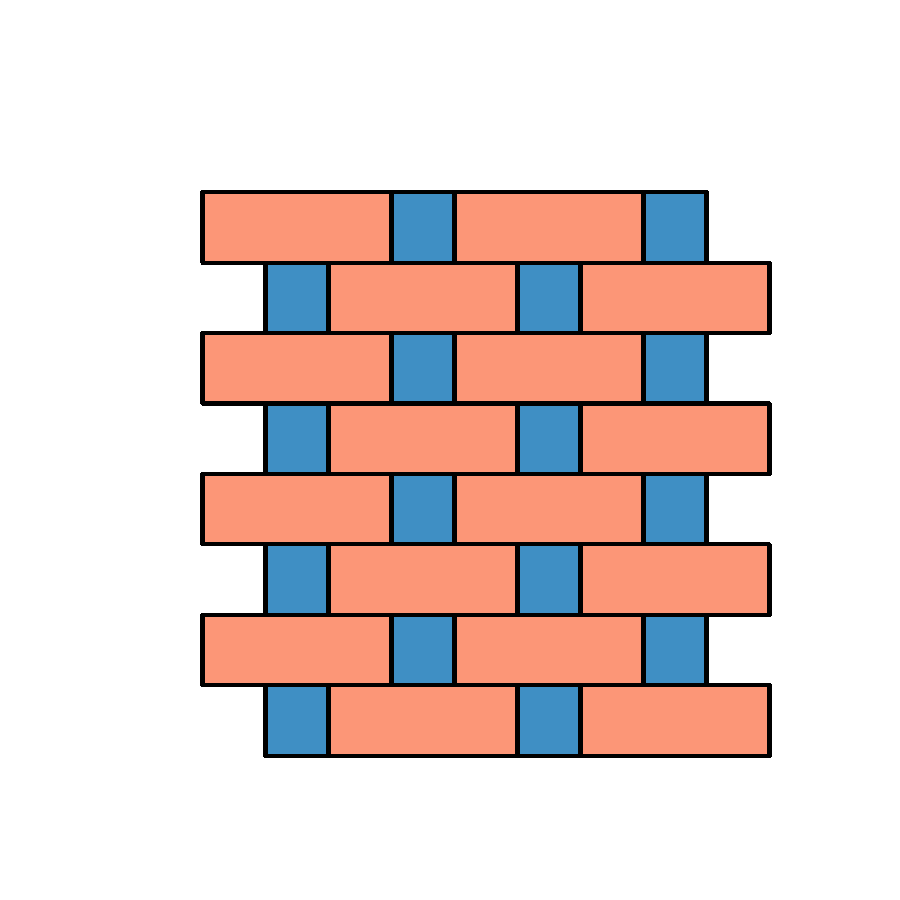
\includegraphics[width=\textwidth]{./figures/procrystals/t6.pdf}
         \caption{}
         \label{fig:pro3pksq3}
     \end{subfigure}
     \hfill
        \begin{subfigure}[b]{0.16\textwidth}
         \centering
         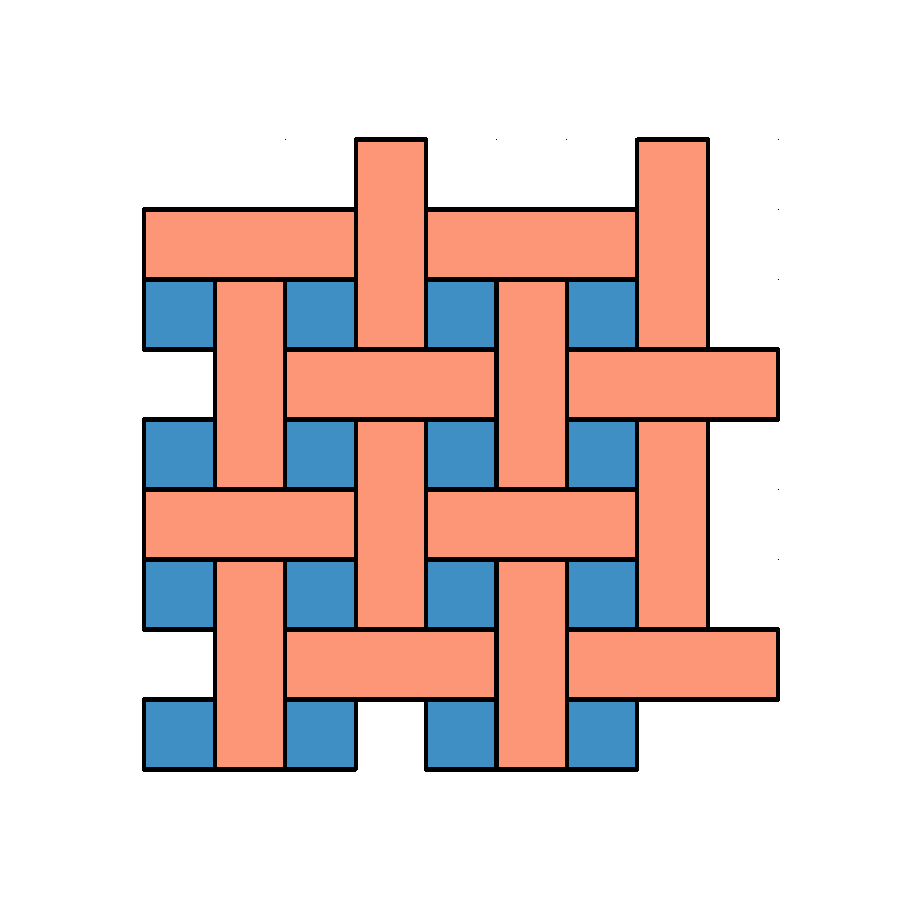
\includegraphics[width=\textwidth]{./figures/procrystals/t3.pdf}
         \caption{}
         \label{fig:pro3pksq4}
     \end{subfigure}
     \hfill
	\vspace{0.5cm}     
          
      \begin{subfigure}[b]{0.16\textwidth}
         \centering
         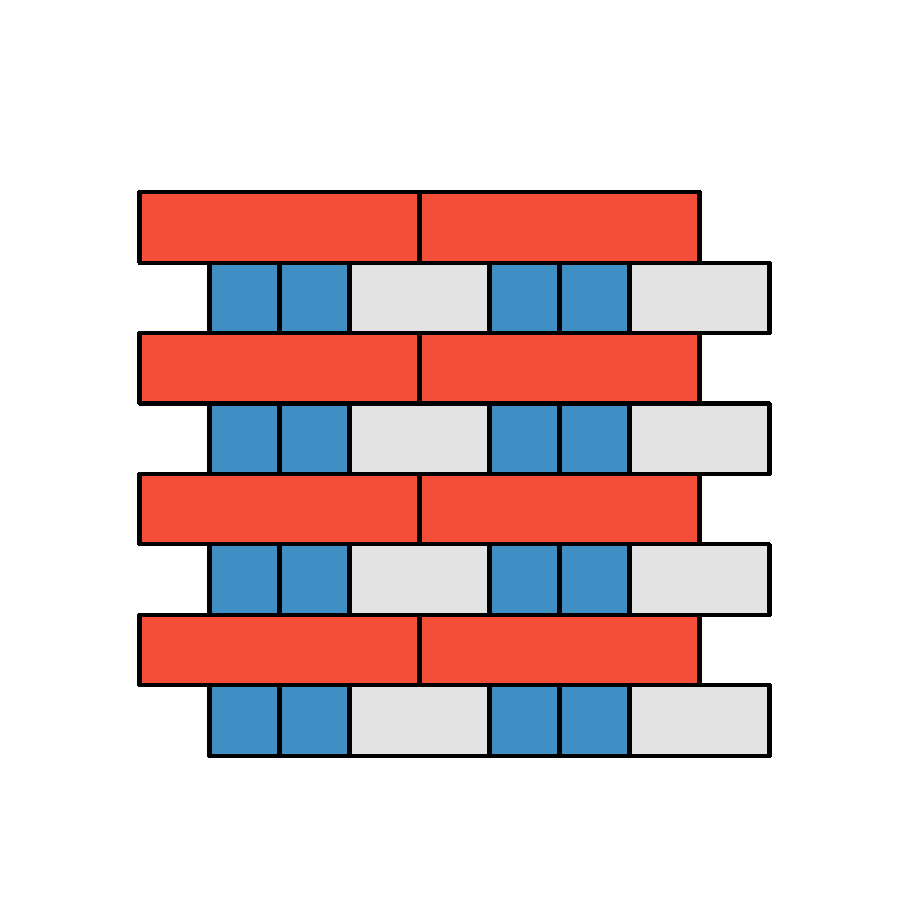
\includegraphics[width=\textwidth]{./figures/procrystals/t2.pdf}
         \caption{}
         \label{fig:pro3pksq5}
     \end{subfigure}
  	\hfill
  	  \begin{subfigure}[b]{0.16\textwidth}
         \centering
         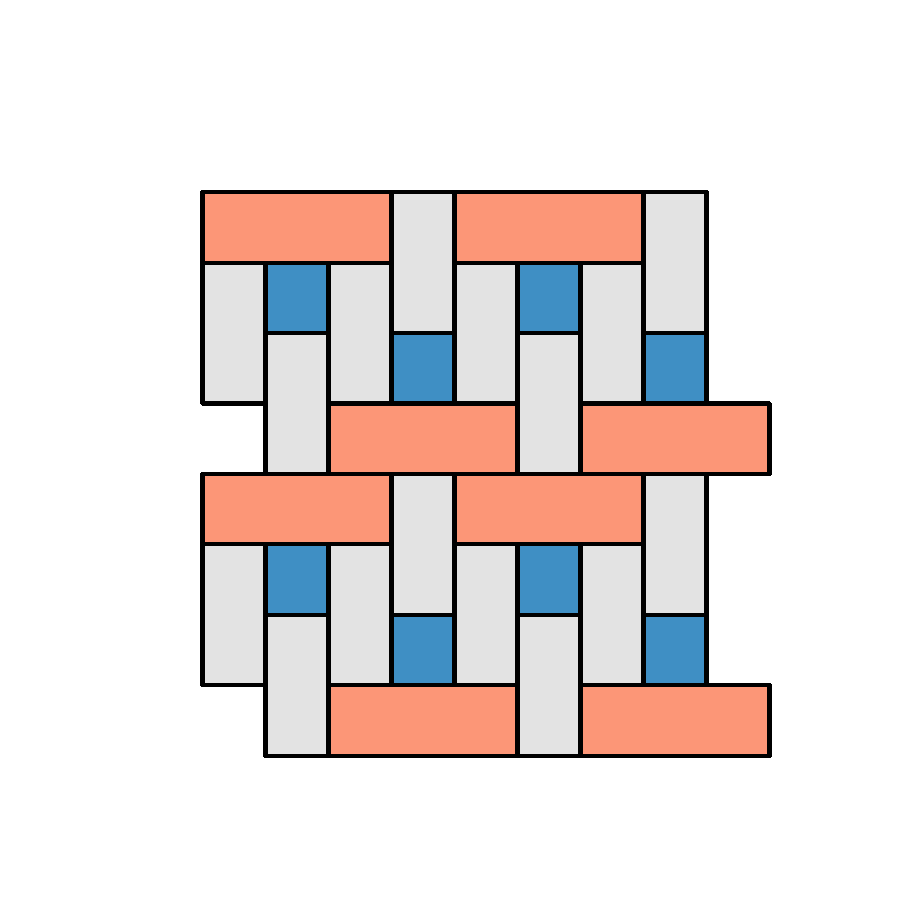
\includegraphics[width=\textwidth]{./figures/procrystals/t5.pdf}
         \caption{}
         \label{fig:pro3pksq6}
     \end{subfigure}
     \hfill
     \begin{subfigure}[b]{0.16\textwidth}
         \centering
         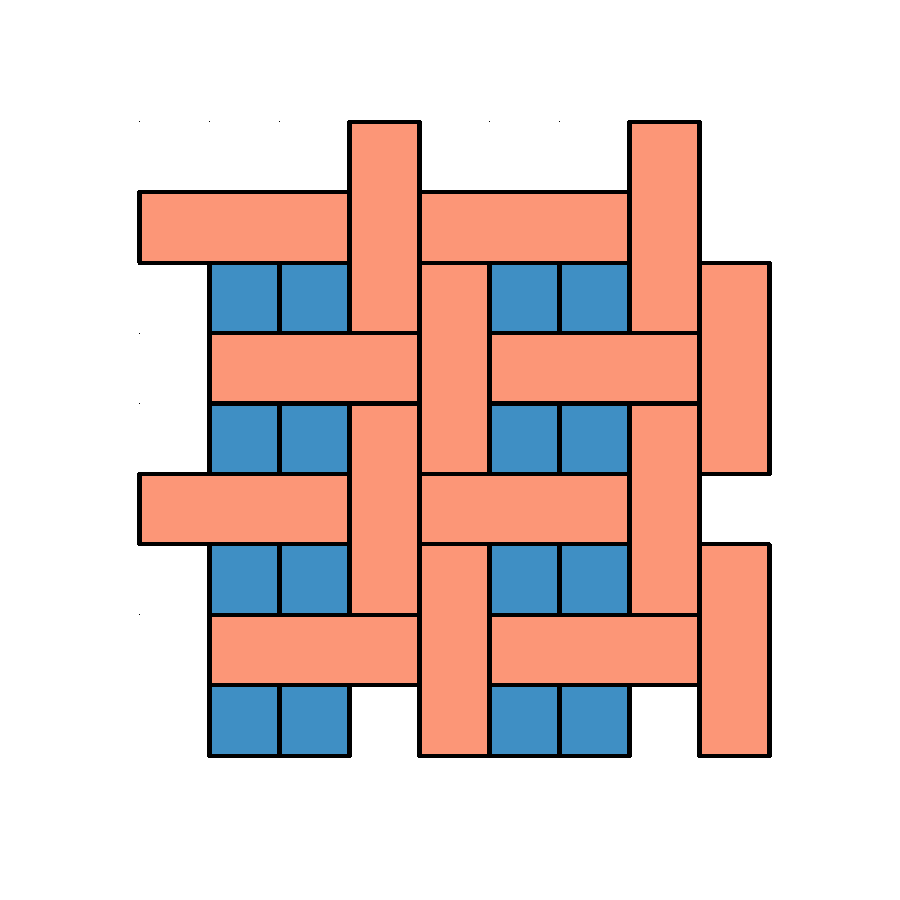
\includegraphics[width=\textwidth]{./figures/procrystals/t0.pdf}
         \caption{}
         \label{fig:pro3pksq7}
     \end{subfigure}
     \hfill
       	 \begin{subfigure}[b]{0.16\textwidth}
         \centering
         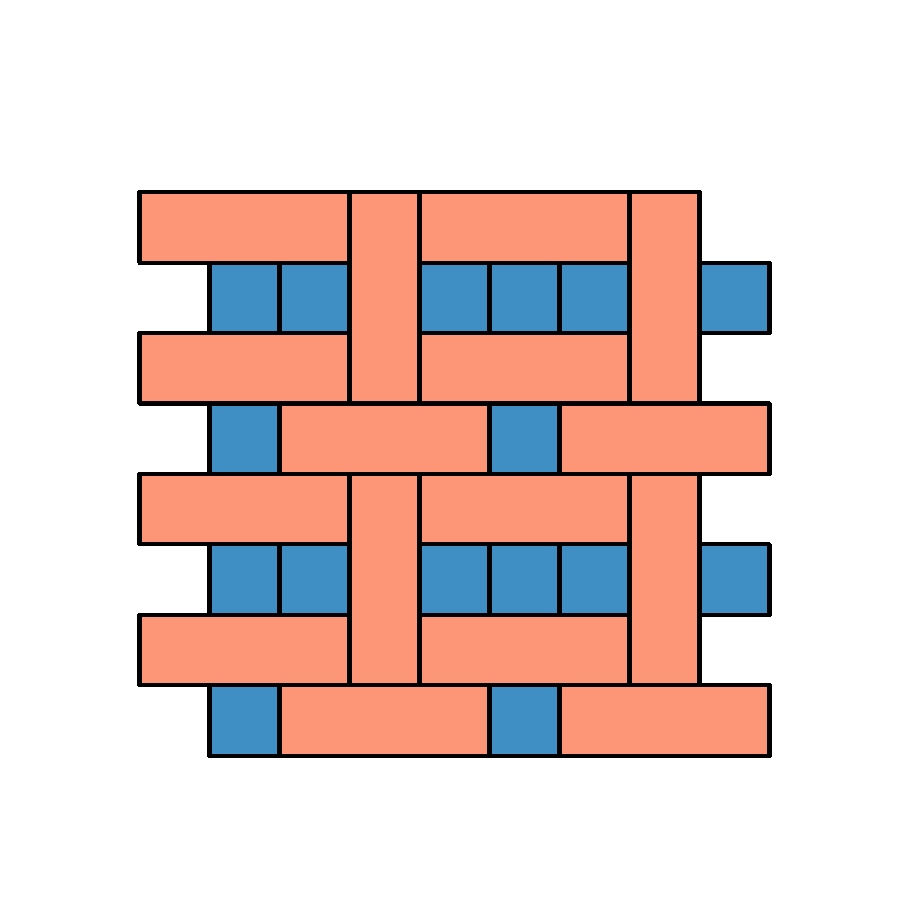
\includegraphics[width=\textwidth]{./figures/procrystals/t1.pdf}
         \caption{}
         \label{fig:pro3pksq8}
     \end{subfigure}
	\hfill      
      \begin{subfigure}[b]{0.16\textwidth}
         \centering
         \includegraphics[width=\textwidth]{./figures/procrystals/t4.pdf}
         \caption{}
         \label{fig:pro3pksq9}
     \end{subfigure}
     \hfill
    
     \caption{The nine unique \pro{4}{3}square lattices for $V=16$, calculated through exact tiling. Four tessellating units are shown for each solution for clarity.}
     \label{fig:pro3pksq}
     
     
     
     \vspace{0.5cm}
      \begin{subfigure}[b]{0.1\textwidth}
         \centering
         \includegraphics[width=\textwidth]{./figures/procrystals/kagome.pdf}
         \caption{}
         \label{fig:pro3pktrihex1}
     \end{subfigure}
     \hfill
      \begin{subfigure}[b]{0.1\textwidth}
         \centering
         \includegraphics[width=\textwidth]{./figures/procrystals/kagome6.pdf}
         \caption{}
         \label{fig:pro3pktrihex2}
     \end{subfigure}
     \hfill
     \begin{subfigure}[b]{0.1\textwidth}
         \centering
         \includegraphics[width=\textwidth]{./figures/procrystals/kagome7a.pdf}
         \caption{}
         \label{fig:pro3pktrihex3}
     \end{subfigure}
     \hfill
     \begin{subfigure}[b]{0.1\textwidth}
         \centering
         \includegraphics[width=\textwidth]{./figures/procrystals/kagome7b.pdf}
         \caption{}
         \label{fig:pro3pktrihex4}
     \end{subfigure}
     \hfill
     \begin{subfigure}[b]{0.1\textwidth}
         \centering
         \includegraphics[width=\textwidth]{./figures/procrystals/kagome7c.pdf}
         \caption{}
         \label{fig:pro3pktrihex5}
     \end{subfigure}
     \hfill
     \vspace{0.2cm}
     
     \begin{subfigure}[b]{0.1\textwidth}
         \centering
         \includegraphics[width=\textwidth]{./figures/procrystals/kagome8a.pdf}
         \caption{}
         \label{fig:pro3pktrihex6}
     \end{subfigure}
     \hfill
     \begin{subfigure}[b]{0.1\textwidth}
         \centering
         \includegraphics[width=\textwidth]{./figures/procrystals/kagome8b.pdf}
         \caption{}
         \label{fig:pro3pktrihex7}
     \end{subfigure}
     \hfill
     \begin{subfigure}[b]{0.1\textwidth}
         \centering
         \includegraphics[width=\textwidth]{./figures/procrystals/kagome8c.pdf}
         \caption{}
         \label{fig:pro3pktrihex8}
     \end{subfigure}
     \hfill
 \begin{subfigure}[b]{0.1\textwidth}
         \centering
         \includegraphics[width=\textwidth]{./figures/procrystals/kagome8d.pdf}
         \caption{}
         \label{fig:pro3pktrihex9}
     \end{subfigure}
     \hfill
     \begin{subfigure}[b]{0.1\textwidth}
         \centering
         \includegraphics[width=\textwidth]{./figures/procrystals/kagome9.pdf}
         \caption{}
         \label{fig:pro3pktrihex10}
     \end{subfigure}
     \hfill
    
     \caption{Units which can be used to rationalise the ring statistics of the \pro{4}{3}trihexagonal lattice. Panel (a) shows a small $V=12$ unit of kagome whilst panels (b)\--(j) show all possible manifestations of a 6\-- (b), 7\-- (c)\--(e), 8\-- (f)\--(i) and 9\-- (j) ring. The numbers in the ring centres indicate the relative degeneracies for each structure.} 
     \label{fig:pro3pktrihex}
\end{figure}

\begin{table}[bt]
\centering
     \caption{The fraction of rings of sizes $k=\{4,6,8,10\}$ for the square lattice
with $V=16$ for the configurations (labelled a-i) shown in figure 
\ref{fig:pro3pksq}. $W$ represents the degeneracy of each configuration and hence its weighting in any
summation.}
\label{tab:sqV16}
%     \begin{tabular}{cccccc}
%     \toprule
%     Config. & $p_4$ & $p_6$ & $p_8$ & $p_{10}$ & $W$ \\
%     \midrule
%     a & 0 & 1 & 0 & 0 & 4 \\
%     b & 0 & 1 & 0 & 0 & 8 \\
%     c & $\frac{1}{2}$ & 0 & $\frac{1}{2}$ & 0 & 8 \\
%     d & $\frac{1}{2}$ & 0 & $\frac{1}{2}$ & 0 & 8 \\
%      e & $\frac{1}{2}$ & $\frac{1}{4}$ & 0 & $\frac{1}{4}$ & 16 \\
%     f & $\frac{1}{4}$ & $\frac{1}{2}$ & $\frac{1}{4}$ & 0 & 32 \\
%     g & $\frac{1}{2}$ & 0 & $\frac{1}{2}$ & 0 & 32 \\
%     h & $\frac{1}{2}$ & 0 & $\frac{1}{2}$ & 0 & 32 \\
%     i & $\frac{3}{8}$ & $\frac{3}{8}$ & $\frac{1}{8}$ & $\frac{1}{8}$ & 64 \\

     \begin{tabular}{cccccccccc}
     \toprule
      Config. & a & b & c & d & e & f & g & h & i\\
     \midrule
	$p_4$ & 0 & 0 & $\frac{1}{2}$ & $\frac{1}{2}$ & $\frac{1}{2}$ & $\frac{1}{4}$ & $\frac{1}{2}$ & $\frac{1}{2}$ & $\frac{3}{8}$ \\[0.5em]
		$p_6$ & 1 & 1 & 0 & 0 & $\frac{1}{4}$ & $\frac{1}{2}$ & 0 & 0 & $\frac{3}{8}$ \\[0.5em] 
		$p_8$ & 0 & 0 & $\frac{1}{2}$ & $\frac{1}{2}$ & 0 & $\frac{1}{4}$ & $\frac{1}{2}$ & $\frac{1}{2}$ & $\frac{1}{8}$ \\[0.5em]
		$p_{10}$ & 0 & 0 & 0 & 0 & $\frac{1}{4}$ & 0 & 0 & 0 & $\frac{1}{8}$ \\[0.5em]
		$W$ & 4 & 8 & 8 & 8 & 16 & 32 & 32 & 32 & 64 \\
     \bottomrule     
     
     \end{tabular}
\end{table}

The \pro{4}{3}trihexagonal lattice is clearly the most constrained system, and is simple enough to fully explain analytically.
Consider a trihexagonal lattice with $V$ nodes. 
This parent lattice must have $2V$ edges and $V$ faces by Euler's formula \davidnote{ref}, $\frac{2V}{3}$ of which are triangles.
Generating the procrystal requires removal $\frac{V}{2}$ edges leaving $\frac{V}{2}$ faces.
Each edge removed must necessarily remove exactly one triangle so that the final number of triangles is $\frac{V}{6}$.
Hence the \pro{4}{3}trihexagonal lattice \textit{must} have $p_3=\frac{1}{3}$.
In addition, this process only allows for rings of size $k=\{3,6,7,8,9\}$ in the final procrystal.
The remainder of the ring statistics can be deduced as follows.
Figure \ref{fig:pro3pktrihex1} shows a small unit of the kagome lattice, and figures \ref{fig:pro3pktrihex2}\--\ref{fig:pro3pktrihex10} the possible resulting procrystalline motifs, with the central number indicating the number of symmetry related species for each motif. 
This analysis predicts a ratio of $1:15:15:1$ for $p_6\rightarrow p_9$, leading to ring statistics of $p_3=\frac{1}{3}$, $p_6=\frac{1}{48}$, $p_7=\frac{15}{48}$, $p_8=\frac{15}{48}$, $p_9=\frac{1}{48}$.
As can be seen in figure \ref{fig:pro3pkb} these are indeed the ring statistics observed for all but the smallest lattice.
Again in the $V=12$ case the $6$\-- and $9$\--rings cannot be supported and so a uniform distribution results (as must be the case for $p_3$ and $\ki=6$). 

For procrystals with higher parent lattice coordinations, in general the ring statistics become more like the ME solutions on moving from an underlying $4$\-- to $5$\-- to $6$\--coordinate lattice, reflecting the decrease in constraints along that pathway.
Furthermore, the subtleties in the ring statistics for these become more difficult to rationalise, reflective of the increased degrees of freedom.
\davidnote{link to later?}
There are some similarities between the different ring distributions.
For example, the snub\--square and triangular lattices (figures \ref{fig:pro3pkd} and \ref{fig:pro3pke}) both show
fewer 4\-- and 5\--membered rings, and more 6\-- and 7\--membered rings, when compared to the ME solutions.
It is interesting to note that distributions of this general form (\ie{} dominated by 3\--rings and large rings) have been observed previously, for example, for a model using a core-softened potential and long-range repulsions \cite{Camp2003}, and for models of BN nanotubes encased in amorphous material \cite{Griebel2007}.
Finally, figure \ref{fig:pro3pkf} shows the ring statistics from the bond switching algorithm (and hence corresponding to a high temperature CRN). 
It is clear that the configurations generated with the procrystalline constraints are fundamentally different purely in terms of the underlying ring statistics.

\subsection{\lm's Law and Assortativity}

In addition to the explicit ring statistics, 3\--coordinate procrystals can be compared to crystals and CRNs through the second moment of the ring statistics and the assortativity.
These are given in figures \ref{fig:pro3p6mu2} and \ref{fig:pro3p6r} respectively.
In addition average values are given in figures \ref{fig:pro3p6ssmu2} \ref{fig:pro3p6ssr} as a function of system size.
Before examining the procrystals, the comparative systems can be discussed.
The crystalline lattices have well defined ring statistics that are not governed by \lm's law but rather by $\mu_2=2\left(1-p_6\right)$ and $\mu_2=4\left(1-\mu_2\right)$, for $8-6^i-5^2$ and $8-6^i-4$ respectively. 
Measuring the ring\--ring correlations through the assortativity is slightly contrived for crystals but can still be done for illustrative purposes and one generally finds highly negative values, indicative of the structural ordering (\davidnote{calculations in appendix}).
In the other extreme, the CRNs generated at infinite temperature lie on the \lm{} curve around the point of highest entropy \ie{} with $p_6\approx 0.105$, due to the effective removal of the enthalpic consideration.
The assortativity for these systems is likewise closer to the random limit of $r=0$.

\begin{figure}[bt]
     \centering
     
     \begin{subfigure}[b]{0.37\textwidth}
         \centering
         \includegraphics[width=\textwidth]{./figures/procrystals/pro3_p6_mu2.pdf}
         \caption{}
         \label{fig:pro3p6mu2}
     \end{subfigure}
     \hfill
     \begin{subfigure}[b]{0.61\textwidth}
         \centering
         \includegraphics[width=\textwidth]{./figures/procrystals/pro3_p6_r.pdf}
         \caption{}
         \label{fig:pro3p6r}
     \end{subfigure}
     
     \begin{subfigure}[b]{0.37\textwidth}
         \centering
         \includegraphics[width=\textwidth]{./figures/procrystals/pro3_ss_mu2.pdf}
         \caption{}
         \label{fig:pro3p6ssmu2}
     \end{subfigure}
     \hfill
        \begin{subfigure}[b]{0.6\textwidth}
         \centering
         \includegraphics[width=\textwidth]{./figures/procrystals/pro3_ss_r.pdf}
         \caption{}
         \label{fig:pro3p6ssr}
     \end{subfigure}
     
     \caption{Panels (a) and (b) plot the second moment of the ring statistics, $\mu_2$, against the assortativity, $r$, respectively for the largest lattice dimension investigated for each procrystal, as well as for selected crystals and CRNs. Panels (c) and (d) plot these same average values for procrystals of increasing lattice dimensions to highlight any system size effects.}
     \label{fig:pro3p6mu2r}
\end{figure}

For four procrystalline lattices (excepting the \pro{4}{3}trihexagonal case) the width of the ring size distribution, as characterised by the second moment, increases as $p_6$ decreases. 
The four cases lie towards the high\--$\mu_2$ limit of the \lm{} curve similar to CRNs, as the formation of arbitrarily large rings is not precluded on enthaplic grounds. 
The \pro{4}{3}square lattice configurations show $\mu_2$ values systematically higher than those predicted from the \lm{} curve. 
For the five-coordinate lattices the \pro{5}{3}snub\--square lattice can be found at $\mu_2$ values significantly higher than those associated with the \lm{} curve (although less removed than those
associated with the \pro{4}{3}square lattice), whilst the \pro{5}{3}elongated\--triangular lattice lies at high $\mu_2$, again
above the \lm{} curve. 
The second moments generated from the triangular lattice lie closest to the low $p_6$ ME limit of $p_6\approx{0.105}$, occupied by the CRNs. 
The exceptional case is once again the \pro{4}{3}trihexagonal procrystal, which has a very well defined $\mu_2$ as a consequence of the constraints on the underlying ring statistics.
The configurations generated on the trihexagonal lattice are unique here in lying at both a low $p_6$ and a relatively low $\mu_2$, and much more in-keeping with systems constrained so as to preclude the formation of large rings (for example, the \td{} crystal constructed purely from $4$\-- and $8$\--membered rings).

The deviation of the second moments from the \lm{} curve is therefore correlated with the strength of the constraints imposed by the underlying crystalline lattice (which decrease from 4\-- to 5\-- to 6\--coordinate).
To reiterate, whilst crystalline lattices are free to locate around the \lm{} curve (their formation usually driven by the energetic landscape), and disordered CRNs constrained to lie upon it; procrystals occupy a region in between these extremes, with the degree of deviation related to the difference in the coordination number of the procrystal and the  underlying lattice.
This contrasts with previous chapters where it was demonstrated how a very wide range of systems (including atomistic networks, colloidal packings, geopolitical maps {\it etc}) generated datasets which did fit on the \lm{} curve.
The configurations generated here are relatively rare examples of systems which do not.

For the assortativities shown in figure \ref{fig:mu2_r_p6}(b), again four of the lattices show similar mean values ($\langle r \rangle\approx -0.19$) corresponding to favouring disassortative configurations. 
Once again it can be noted that these procrystals occupy the space between crystalline and amorphous systems.
Similar to previous observations, the \pro{4}{3}trihexagonal lattice is unique in displaying highly disassortative and well\--defined behaviour, with $\langle r \rangle \approx -0.275$.
Careful observation of figure \ref{fig:pro3pktrihex} allows the joint degree distribution to be explicitly written as \davidnote{need appendix on this?}:
\begin{equation}
	\mathbf{e} = \frac{1}{96}\: \begin{blockarray}{*{5}{c} l}
	\begin{block}{*{5}{>{$\footnotesize}c<{$}} l}
	3 & 6 & 7 & 8 & 9 \\
	\end{block}
	\begin{block}{[*{5}{c}]>{$\footnotesize}l<{$}}
	0 & 0 & 5 & 10 & 1\: \bigstrut[t]& \:3\\
	0 & 0 & 1 & 1 & 0 & \:6 \\
	5 & 1 & 14 & 14 & 1 & \:7\\
	10 & 1 & 14 & 14 & 1 & \:8\\
	1 & 0 & 1 & 1 & 0 & \:9\\
	\end{block}
	\end{blockarray}\,.
\end{equation} 
This corresponds to $r=-101/367\approx -0.275$, as measured from simulation.

System size effects for the procrystalline lattices are provided in figures \ref{fig:pro3p6ssmu2} \ref{fig:pro3p6ssr}.
As can be seen, there is often a relatively large change initially, as certain ring sizes or motifs cannot be accommodated due to the restrictions in lattice size (as previously discussed).
However, both metrics appear to be converging as lattice size is scaled.
\davidnote{discuss}